\chapter{Experimentelle Resultate und Analysen}
\label{chapter:experiment}

Im Folgenden sollen die im Rahmen dieser Arbeit aufgenommenen Daten vorgestellt und ausgewertet werden. Dabei lassen sich diese in zwei separate Bemühungen unterteilen. Zum einen wurden Untersuchungen zur Dynamik in CRN angestellt, welche zuerst präsentiert werden sollen, zum anderen wurde die Linienformänderungen in Abhängigkeit der Temperatur untersucht und mit theoretischen Überlegungen verglichen.

Im Verlauf der Auswertung werden die Daten teil nach dem verwendeten Spektrometer unterschieden. Dies liegt an der unterschiedlichen Larmorfrequenzen, $\omega_{L, \text{OBI}} = 2\pi \cdot \SI{97.1722}{MHz}$ im Vergleich zu $\omega_{L, \text{Bruker}} = 2\pi \cdot \SI{130.9736}{MHz}$ der Apparaturen, welche sich um etwa einen Faktor $\SI{1.35}{}$ unterscheiden -- genug um eine deutliche Auswirkung in den Daten beobachten zu können.

Bei beiden Spektrometern wurden für die grundlegenden Parameter bei allen Messungen etwa die gleichen Einstellungen verwendet: Für das OBI-Spektrometer wurde die Dauer eines $\SI{180}{\degree}$-Pulses auf einen Wert zwischen $\SI{6.5}{\micro s}$ und $\SI{7.1}{\micro s}$ gesetzt, beim Bruker-Spektrometer auf $\SI{5.2}{\micro s}$. Die Evolutionszeit $t_p$ der Echos beträgt in den meisten Fällen $\SI{15}{\micro s}$ und nie mehr als $\SI{20}{\micro s}$. Die Wiederholungszeit, also die Zeit zwischen zwei Pulsfolgen beträgt etwa $\SI{10}{\milli s}$. Der mit dem OBI-Spektrometer abgedeckte Temperaturbereich reicht von $\SI{230}{\kelvin}$ bis $\SI{435}{\kelvin}$, während sich der Temperaturbereich des Bruker-Spektrometers auf den Bereich von $\SI{310}{\kelvin}$ bis $\SI{390}{\kelvin}$ beschränkt.

Alle erwähnten Fits wurden durch eine least-squares-Methode erstellt.


\section{Bestimmung von $T_1$ und $T_2$} \label{section:res:T_1}

Vor dem Beginn jeder NMR-Messung ist es sinnvoll, $T_1$ im zu untersuchenden Temperaturgebiet zu vermessen. Dies ist hilfreich um wichtige Parameter der Messungen abzustecken und mögliche Hindernisse im Vorhinein erahnen zu können. So sollte zwischen allen Messungen eine Zeit von mindestens $4 T_1$ gewartet werden, um sicherzugehen, dass sich die Magnetisierung in guter Näherung wieder im Gleichgewichtszustand befindet. Wird $T_1$ also im Laufe der Messung bei anderen Temperaturen länger, muss hierauf Rücksicht genommen werden. Wird $T_1$ auf der anderen Seite sehr kurz, kann es passieren, dass Signale sehr schnell zerfallen und den Experimentierenden mit einem schlechten Signal-Rausch-Verhältnis zurücklassen. Hinzu kommt, dass der Verlauf von $T_1$ nach Formel \eqref{eqn:bpp} wertvolle Information über die Dynamik in der untersuchten Probe liefern kann. Zuletzt bietet diese recht einfache und reproduzierbare Messung die Möglichkeit, den Aufbau und die Probe auf Übereinstimmung mit Literaturdaten hin zu überprüfen. Daher wurden zu allen untersuchten Temperaturen $T_1$-Messungen aufgenommen.

Zur Bestimmung von $T_1$ wurde eine Invertierungs-Pulsfolge mit Hahn-Echo verwendet.

Repräsentative Rohdaten einer solchen Messung sind in Abbildung \ref{fig:res:T_1_roh} zu sehen. An die Daten wurden Fits mit $T_1$ und $\beta$ als freien Parametern entsprechend Gleichung \eqref{eqn:theo:T_1_fit} angelegt -- diese sind als Linien dargestellt. Die Daten wurden hier zudem auf den Bereich zwischen $1$ und $-1$ normiert, um einen besseren Vergleich zuzulassen. Es ist zu erkennen, dass die Fits eine gute Repräsentation der Daten ermöglichen.
\begin{figure}
	\begin{center}
		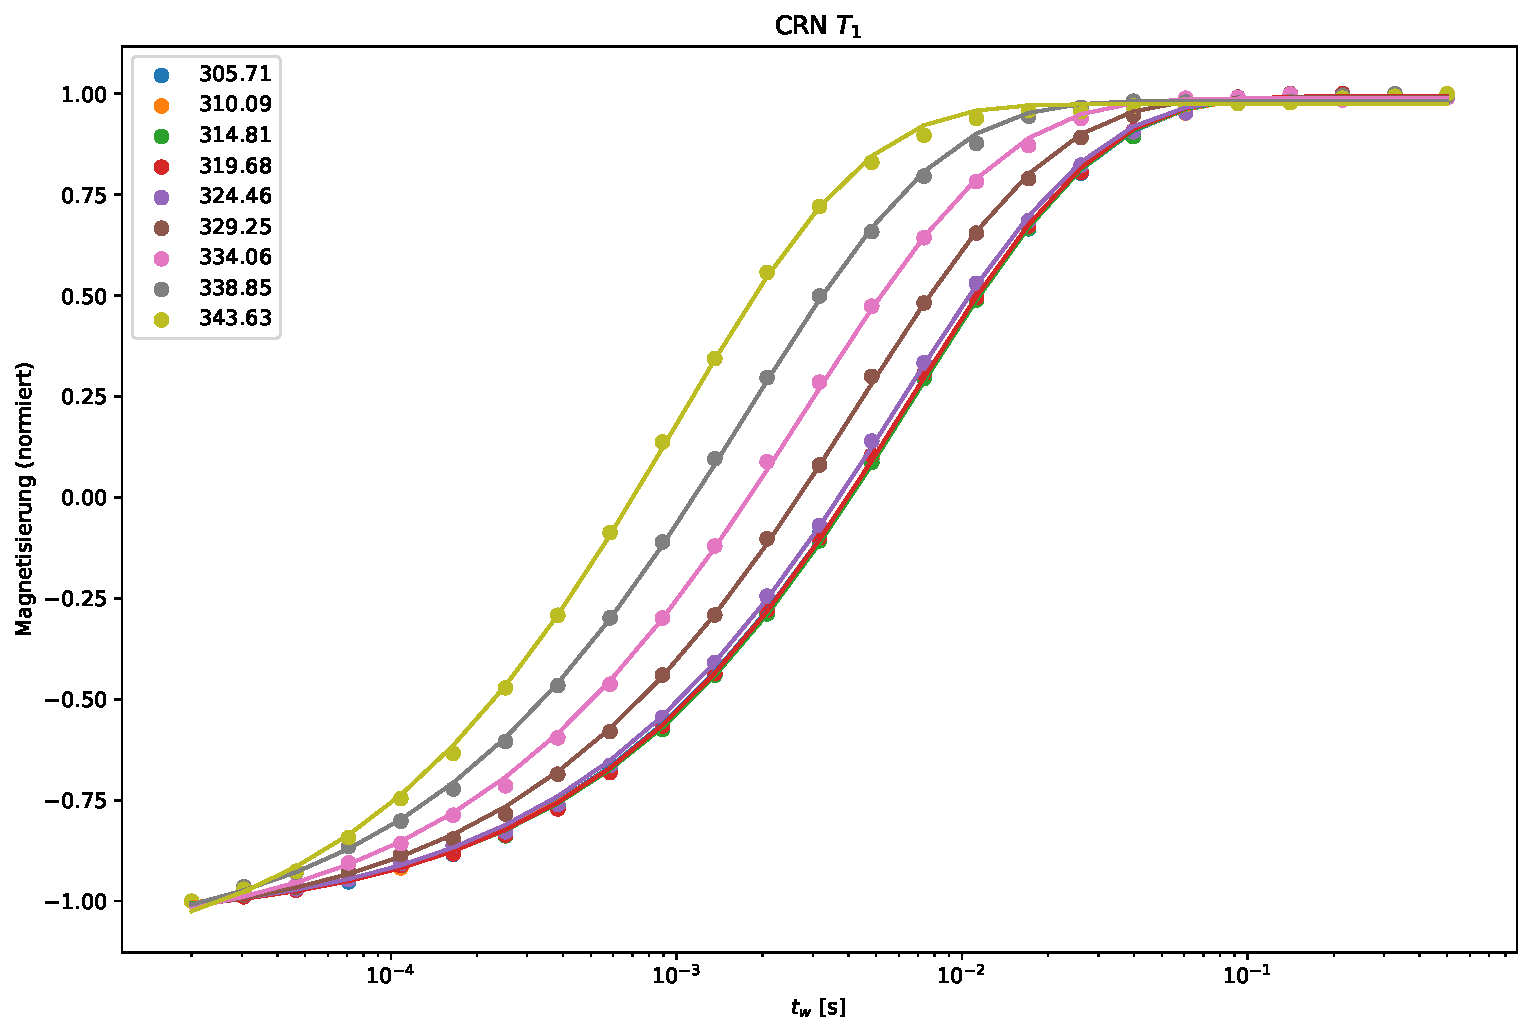
\includegraphics[width=\textwidth]{graphics/plots/T1/t1_roh.pdf}
	\end{center}
	\caption{Normierte $T_1$ Rohdaten. Linien stellen Fits an die Datenpunkte dar.} \label{fig:res:T_1_roh}
\end{figure}

Während sich die Kurven zwischen $\SI{305}{\kelvin}$ und $\SI{325}{\kelvin}$ sehr ähneln, verschieben sich die Kurven und damit auch die $T_1$-Werte bei höheren Temperaturen zu kürzeren Zeiten.

Dies lässt sich auch in der Gesamtübersicht aller aufgenommenen $T_1$-Daten in Abbildung \ref{fig:res:T_1} erkennen. Während die $T_1$-Zeiten bei Temperaturen von $\SI{250}{\kelvin}$ bis $\SI{325}{\kelvin}$ nahezu unverändert im unteren Millisekunden-Bereich liegen, verkürzen sie sich bei steigenden Temperaturen bis in den zweistelligen Mikrosekunden-Bereich. Es ist ein $T_1$-Minimum bei etwa $\SI{390}{\kelvin}$ mit einem Wert von ungefähr $\SI{20}{\micro s}$ auszumachen, ehe die $T_1$-Zeiten stagnieren oder sogar länger werden.
\begin{figure}
	\begin{center}
		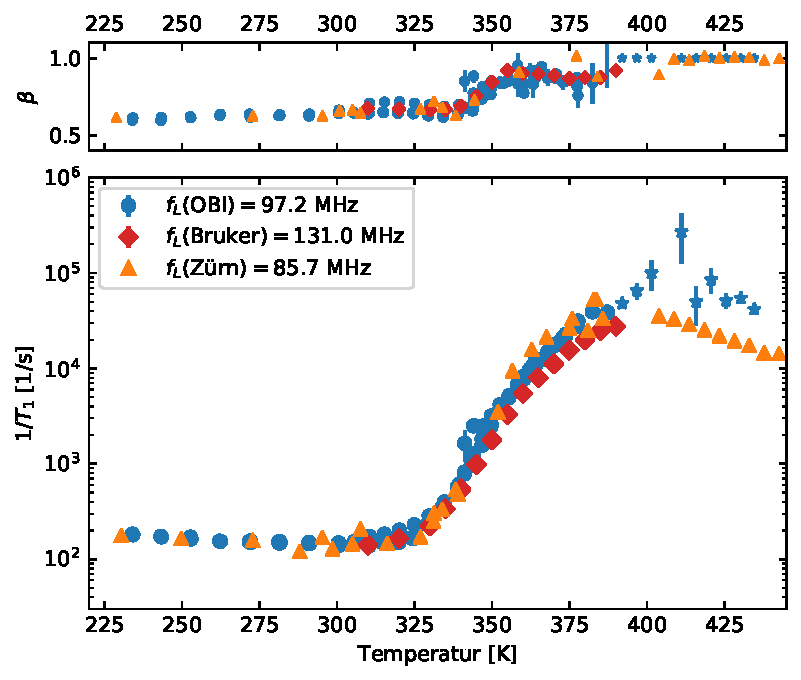
\includegraphics[width=\textwidth]{graphics/plot/t1.pdf}
	\end{center}
	\caption{$T_1$ und $\beta$ aus Fits nach Gleichung \eqref{eqn:theo:T_1_fit}. Blaue und rote Symbole indizieren die am OBI- bzw. Bruker-Spektrometer aufgenommen Daten; orangene Kreuze bieten einen Vergleich mit Daten von Zürn \cite{zuern_paper}.} \label{fig:res:T_1}
\end{figure}

Während die Unsicherheiten weitestgehend vernachlässigbar sind und die größe der dargestellten Symbole nicht überschreiten, sind starke Schwankungen über $\SI{390}{\kelvin}$ zu erkennen. Einem Großteil der dort aufgenommenen Daten kann nicht mehr Bedeutung als einer groben Idee der Tatsachen zugemessen werden.

Abgesehen von dem erwähnten Temperaturbereich ist eine gute Übereinstimmung zu den $T_1$-Daten von Zürn \cite{zuern_paper} und zwischen mehrfach durchgeführten Messungen mit überlappenden Temperaturbereichen zu erkennen, was darauf schließen lässt, dass diese Daten gut reproduzierbar sind. Die am Bruker-Spektrometer aufgenommenen Daten folgen dem gleichen, beschriebenen Verlauf und zeigen bis auf den Temperaturbereich zwischen $\SI{360}{\kelvin}$ und $\SI{390}{\kelvin}$ keinen nennenswerte Differenzen; dort aber sind die gemessenen $T_1$-Daten zu leicht längeren Zeiten verschoben. Der Quotient der $T_1$-Zeiten überschreitet den Wert $\SI{2}{}$ jedoch nicht.

Im oberen Teil der Abbildung \ref{fig:res:T_1} sind die entsprechenden $\beta$ der Fits zu sehen. Von einem Wert von $\SI{0.6}{}$ bei tieferen Temperaturen steigen sie zu einem Wert von etwa $\SI{0.9}{}$ bei Temperaturen über $\SI{350}{\kelvin}$. Dies entspricht etwa den Ergebnissen von Zürn.

Abweichungen gibt es lediglich bei den höheren Temperaturen, wo $\beta$ laut \cite{zuern_paper} nahe $\SI{1.0}{}$ liegt -- welches hier nicht ganz erreicht wird --, allerdings mit größeren Messunsicherheiten, welche auch hier bei Temperaturen über $\SI{350}{\kelvin}$ zu beobachten sind. Werte über $\SI{390}{\kelvin}$ wurden ausgelassen, da die Messunsicherheiten zu groß waren, als dass den Werten eine Aussage zugestanden werden könnte. Diese stammen daher, dass mit den verwendeten Apparaturen nicht verlässlich Datenpunkte vor $\SI{10}{\micro s}$ aufgenommen werden können. Wenn die $T_1$ Zeit aber in der gleichen Größenordnung liegt und zum Zeitpunkt des $T_1$-Werts das Signal auf etwa $1/e$ abgefallen ist, ist es verständlich, dass ein Fit Schwierigkeiten bereiten kann. Lösen ließe sich dies theoretisch mit einer längeren Evolutionszeit des verwendeten Echos, dies ist aufgrund der kurzen $T_1$- und $T_2$-Zeiten in diesem Temperaturbereich jedoch nicht möglich -- das entstehende Signal ist zu klein um effektiv vom Rauschen getrennt zu werden.

Dennoch ist auffällig, dass trotz der Unsicherheiten von $\beta$ eine relativ gute Übereinstimmung mit den Daten von Zürn vorliegt -- auch von zwei Messreihen zwischen $\SI{315}{\kelvin}$ und $\SI{340}{\kelvin}$ produzierte $\beta$ mit einer Differenz von etwa $\SI{0.1}{}$, sind die entsprechenden $T_1$ in Übereinstimmung miteinander und mit der Literatur. Dies gibt ein Indiz,welche Aussagekraft den exakten Werten von $\beta$ zugemessen werden kann.

Die Unsicherheiten der mit dem Bruker-Spektrometer bestimmten $\beta$ ist vergleichsweise gering. Dies ist mit der höheren Qualität der Daten (besonders auch in Abbildung \ref{fig:res:bruker_linienform} im Vergleich zu \ref{fig:res:spek_linienform} zu erkennen) und den niedrigeren $T_1$-Werten zu erklären.



% \section{$T_2$} \label{section:res:T_2}
\par\bigskip


Ähnlich wie $T_1$ ist auch $T_2$ eine wichtige Größe, die Parameter für folgende Messungen bestimmen kann -- die praktikablen Längen von Echos werden von $T_2$ begrenzt --, oder nach Formel \eqref{eqn:theo:T_2_dyn} Aufschluss über Dynamiken gibt.

In Abbildung \ref{fig:res:T_2_roh} sind exemplarisch Rohdaten verschiedener Temperaturen zu sehen. Diese wurden mit einem Hahn-Echo mit $\tau = \SI{15}{\micro s}$ aufgenommen und auf den Bereich zwischen $\SI{0}{}$ und $\SI{1}{}$ normiert.
\begin{figure}
	\begin{center}
		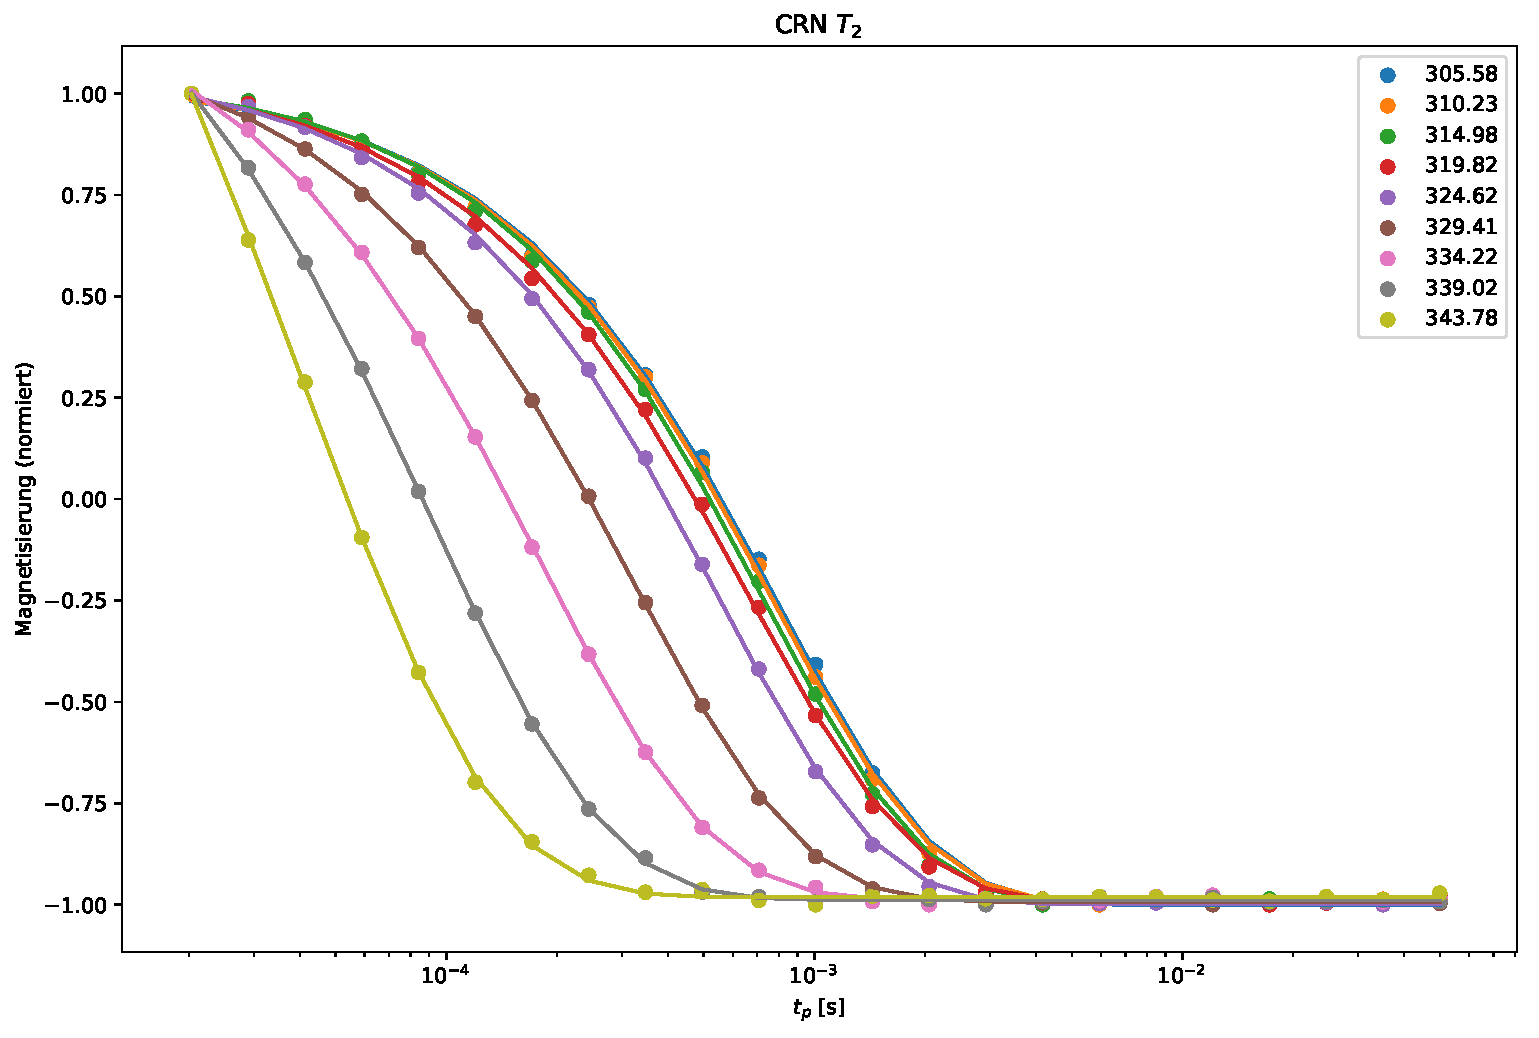
\includegraphics[width=\textwidth]{graphics/plots/T2/t2_roh.pdf}
	\end{center}
	\caption{Normierte $T_2$ Rohdaten. Linien stellen Fits an die Datenpunkte dar.} \label{fig:res:T_2_roh}
\end{figure}

An diese wurden Fit-Funktionen nach \eqref{eqn:theo:T_2_fit} angelegt, welche als Linien dargestellt sind. Es lässt sich mit den Fits eine gute Übereinstimmung zu den Daten erzielen. Auch hier lässt sich erkennen, dass $T_2$ bei Temperaturen bis etwa $\SI{320}{\kelvin}$ nahezu konstant verbleibt, und zu hoheren Temperaturen kleiner wird.

Abbildung \label{fig:res:T_2} zeigt eine Übersicht über die aufgenommen $T_2$-Werte mit den zugehörigen $\beta$ der Fits. Unter $\SI{320}{\kelvin}$ verbleiben erstere im niedrigen Millisekunden-Bereich, ehe sie deutlich kürzer werden und sich bei etwa $\SI{360}{\kelvin}$ ein Minimum zeigt. Die Werte des Bruker-Spektrometers sind hiermit in guter Übereinstimmung, wobei wiederum festzuhalten ist, dass die Messunsicherheiten geringer sind. Ein zweites Minimum zeigt sich bei etwa $\SI{400}{\kelvin}$, dessen Wert sich, ebenso wie der erste, im zweistelligen Mikrosekunden-Bereich befindet. Zwischen $\SI{400}{\kelvin}$ und $\SI{410}{\kelvin}$ ist zu erkennen, dass -- wohl durch die Kürze von $T_2$ bei diesen Temperaturen -- deutlich größere Unsicherheiten als im Rest der Messreihe vorliegen, wo sie in guter Näherung vernachlässigbar sind.
\begin{figure}
	\begin{center}
		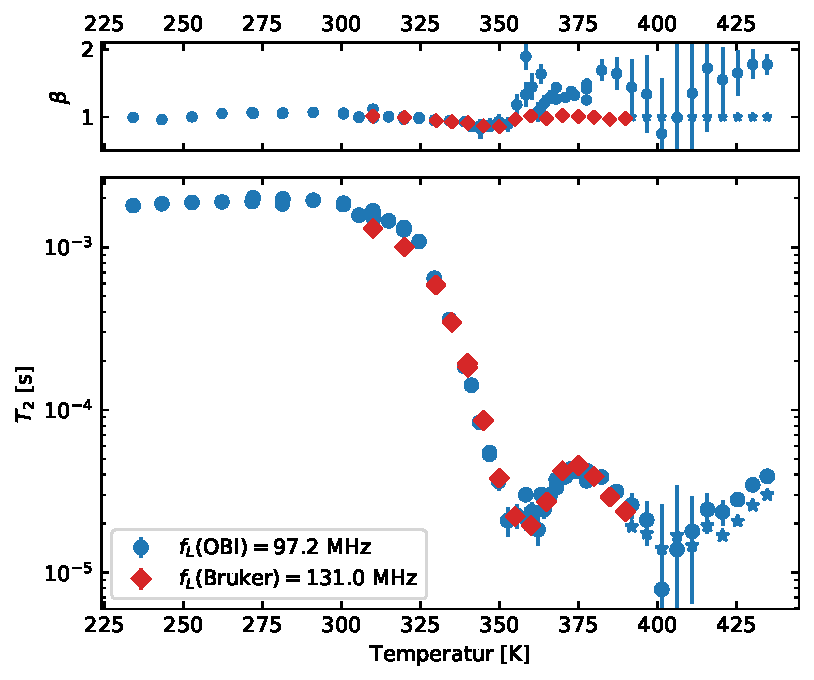
\includegraphics[width=\textwidth]{graphics/plot/t2.pdf}
	\end{center}
	\caption{$T_2$ und $\beta$ aus Fits nach Gleichung \eqref{eqn:theo:T_2_fit}. Blaue und rote Symbole indizieren die am OBI- bzw. Bruker-Spektrometer aufgenommen Daten.} \label{fig:res:T_2}
\end{figure}

Auch die $\beta$-Werte zeigen bei höheren Temperaturen deutlich größere Unsicherheiten, hier allerdings schon zwischen $\SI{390}{\kelvin}$ und $\SI{425}{\kelvin}$, was eine Bestimmung der Werte verkompliziert. Sie scheinen zwischen $\SI{1}{}$ und $\SI{2}{}$ zu liegen. Bei tieferen Temperaturen klärt sich das Bild etwas: Während die Daten des OBI-Spektrometers bei Temperaturen bis $\SI{350}{\kelvin}$ ein $\beta$ zwischen $\SI{1}{}$ und $\SI{1.5}{}$ suggerieren, zeigen die Daten des Bruker-Spektrometers ein $\beta$ um $\SI{1}{}$ -- mit geringerer Unsicherheit. Bei nochmals tieferen Temperaturen scheint $\beta$ konsistent bei rund $\SI{1}{}$ zu liegen.




\section{Dynamik bei stimulierten Echos und $t_p$-abhängigen Spektren} \label{section:res:F_2}

Mit der Absicht einen möglichen Betaprozess zu identifizieren, wurden $F_2$-Messungen, also stimulierte Echos, durchgeführt. Dazu wurden am Spektrometer OBI über eine Reihe von Temperaturen von $\SI{230}{\kelvin}$ bis $\SI{310}{\kelvin}$ und Evolutionszeiten von $\SI{50}{\micro s}$ bis $\SI{1000}{\micro s}$ Messungen durchgeführt. Es wurde eine Drei-Puls-Folge verwendet und so sowohl Cos-Cos- als auch Sin-Sin-Korrelation gemessen.

Die meisten ähnelten der hier beispielhaft ausgewählten Messung bei $\SI{280}{\kelvin}$ und einer Evolutionszeit von $t_p = \SI{1000}{\micro s}$: Die Daten lassen sich schwerlich oder gar nicht von einer $T_1$-Kurve unterscheiden, die bei gleicher Temperatur aufgenommen wurde, wie in Abbildung \ref{fig:res:F_2_tieftemp} zu sehen. Es scheint daher nicht möglich, in diesem Temperaturbereich mit dieser Methode Aussagen über mögliche Dynamik treffen zu können.
\begin{figure}
	\begin{center}
		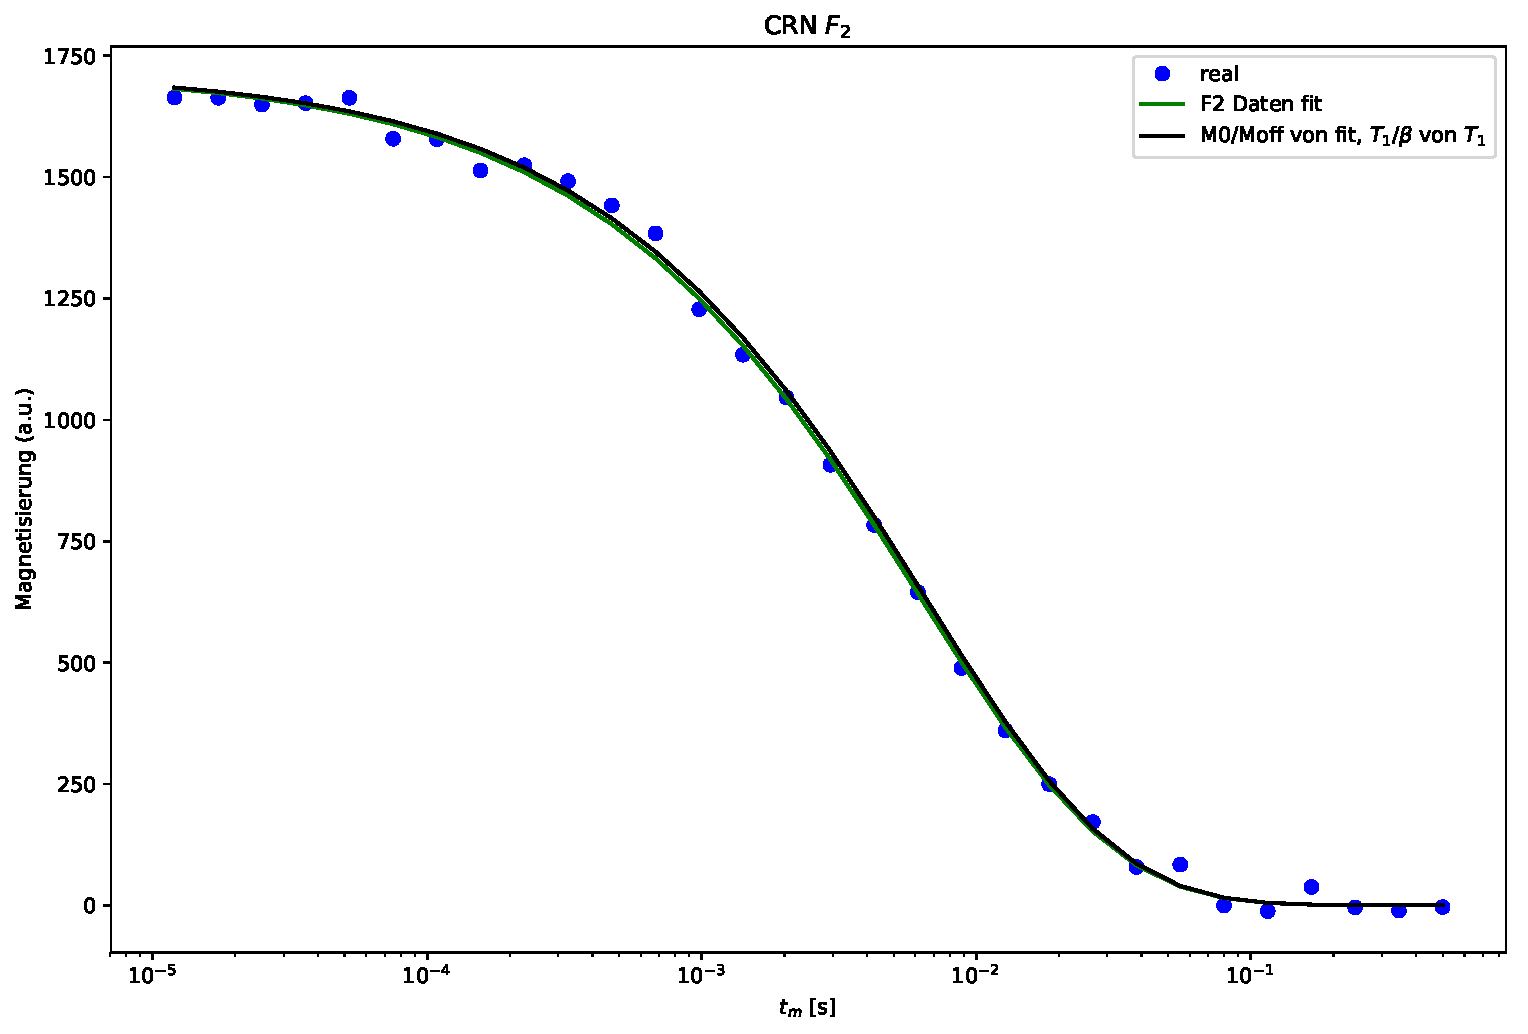
\includegraphics[width=\textwidth]{graphics/plots/F2/f2_tieftemp.pdf}
	\end{center}
	\caption{$F_2$ Messungen bei $\SI{280}{\kelvin}$. Grüne Linie zeigt einen Fit an die Daten, schwarze Linie zeigt den Fit mit der Zeitkonstante und $\beta$ ersetzt durch $T_1$ und $\beta_{T_1}$. Die Kurven sind fast identisch, was heißt, dass die Kurven keine Dynamik außer $T_1$ zeigen.} \label{fig:res:F_2_tieftemp}
\end{figure}

Lediglich bei den Temperaturen $\SI{300}{\kelvin}$ und $\SI{310}{\kelvin}$, sowie $t_p = \SI{1000}{\micro s}$ konnte ein nennenswerter Unterschied zu reinen $T_1$-Kurven beobachtet werden; die entsprechenden Messungen sollen im Folgenden besprochen werden.

Einen Fit der Form *** (Formel) direkt an die Messwerte anzulegen erwies sich als schwierig, daher wurde folgende Schritte für eine Auswertung durchgeführt: An die Daten wurde folgende Funktion gefittet:
\begin{align}
	M_{F_2} (t_m) = M_0 \left[ \exp{ \left(- { \left( \frac{t_m}{F_2} \right) }^{\beta_{F_2}} \right)} \right] + M_\text{off} \label{eqn:res:F_2_fit}
\end{align}
Dieser Fit stellt die grüne Kurve in Abbildung \ref{fig:res:F_2_fit} dar.
\begin{figure}
	\begin{center}
		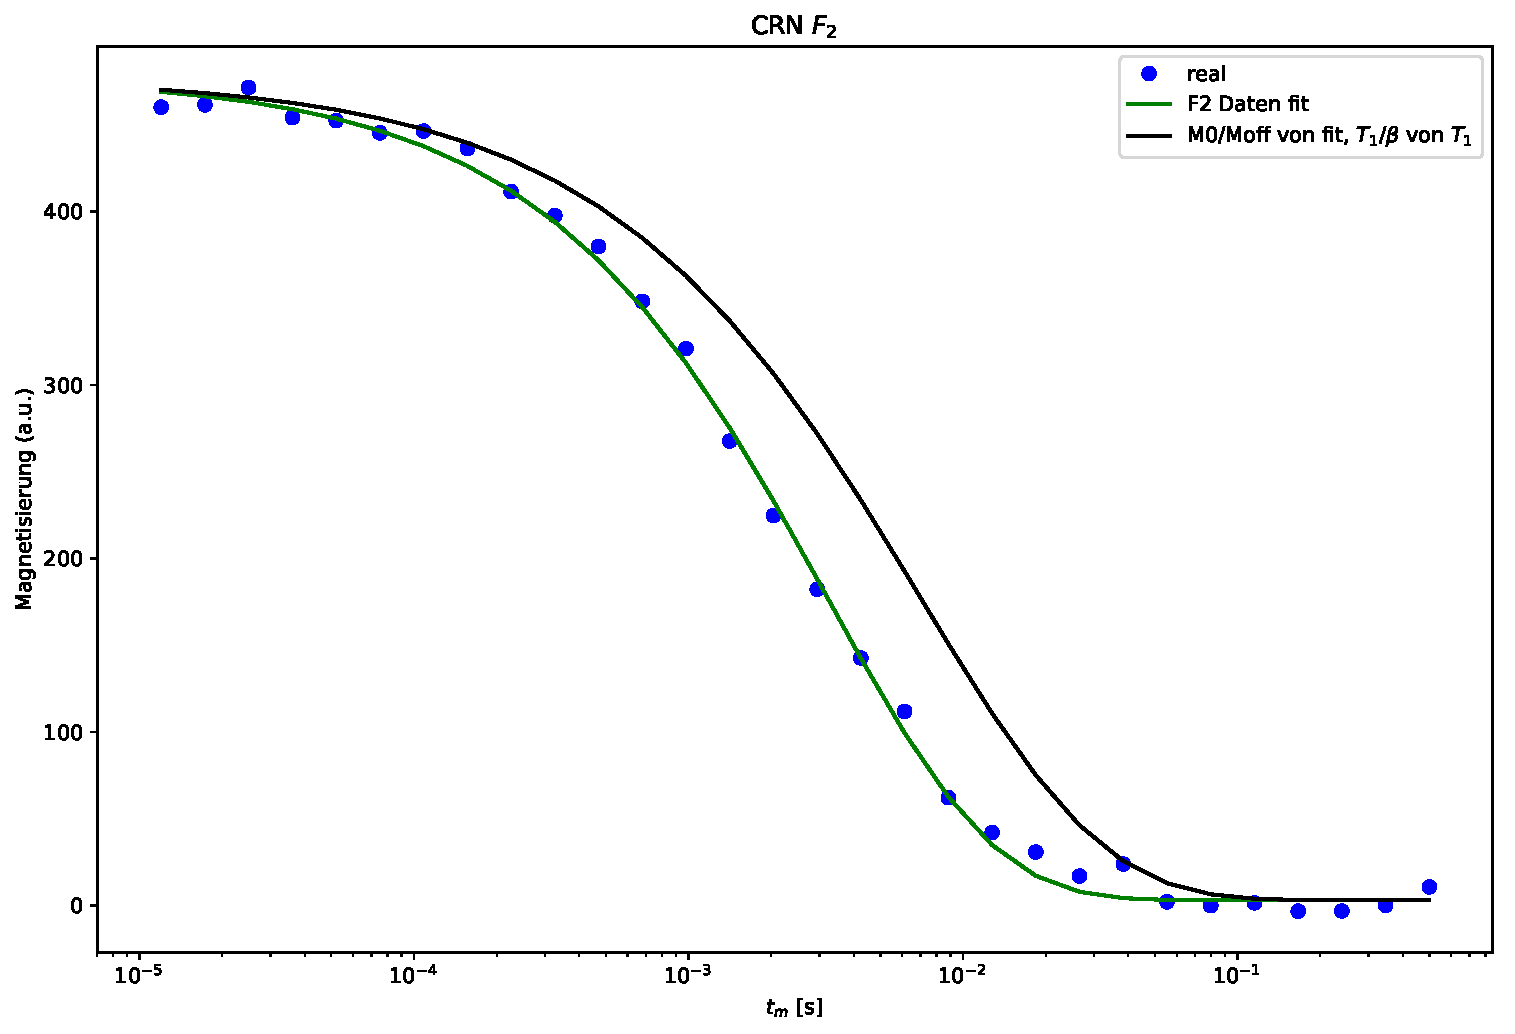
\includegraphics[width=\textwidth]{graphics/plots/F2/f2_fits.pdf}
	\end{center}
	\caption{$F_2$ Messungen bei $\SI{310}{\kelvin}$. Grüne Linie zeigt einen Fit an die Daten, schwarze Linie zeigt den Fit mit der Zeitkonstante und $\beta$ ersetzt durch $T_1$ und $\beta_{T_1}$. Es ist ein deutlicher Unterschied zwischen den Kurven zu erkennen, was auf stattfindende Dynamik hinweist.} \label{fig:res:F_2_fit}
\end{figure}
Die Werte $F_2$ und $\beta_{F_2}$ wurden dann durch $T_1$ und $\beta_{T_1}$ einer $T_1$-Messung gleicher Temperatur ersetzt -- das Resultat ist als schwarze Kurve gezeigt. Dieses Vorgehen macht es möglich, die $T_1$-Kurve an die $F_2$-Daten anzupassen. Es wurden nun die Daten durch die angepasste $T_1$-Kurve geteilt um den entsprechenden Anteil zu eliminieren. Das Resultat ist in Abbildung \ref{fig:res:F_2_T_1} gezeigt.
\begin{figure}
	\begin{center}
		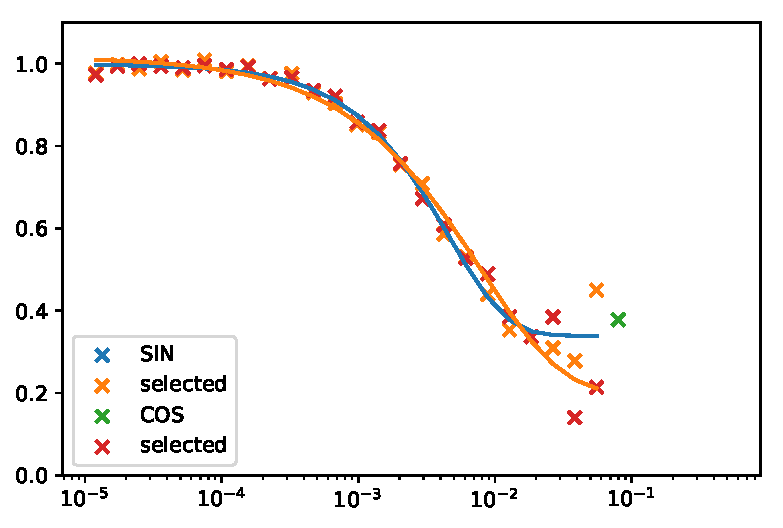
\includegraphics[width=\textwidth]{graphics/plots/F2/f2_fit.pdf}
	\end{center}
	\caption{$F_2$-Daten bei $\SI{310}{\kelvin}$ geteilt durch mit $T_1$ und $\beta_{T_1}$ modifiziertem Fit. An die entstandenden Daten wurden Kohlrausch-Fits (dargestellt als Linien) angelegt um Zeitkonstanten zu gewinnen.} \label{fig:res:F_2_T_1}
\end{figure}

Da die Daten bei Mischzeiten von über $\SI{100}{\milli s}$ stark streuen wurden sie nicht dargestellt. An verbleibenden Punkte wiederum kann ein Kohlrausch-Fit angelegt werden, um über den beschriebenen Umweg zu einer Funktion ähnlich der aus Formel *** zu gelangen.

Es wurden je zwei Messungen einer Cos-Cos-Pulsfolge und einer Sin-Sin-Pulsfolge bei $\SI{310}{\kelvin}$ durchgeführt, sowie je eine Messung bei $\SI{300}{\kelvin}$. Die Resultate finden sich in Tabelle \ref{tab:res:F_2}

\begin{table}[H]
	\centering
	\begin{tabular}{lllll}
		\hline
		Temperatur & Sin-Sin $\tau$ & Sin-Sin $\beta$ & Cos-Cos $\tau$ & Cos-Cos $\beta$ \\ \hline
		$\SI{300}{\kelvin}$ (Lauf 1) & $\SI{5.26 (94)}{\milli s}$ & $\SI{0.95 (18)}{}$ & $\SI{3.68 (63)}{\milli s}$ & $\SI{1.30 (34)}{}$ \\
		$\SI{310}{\kelvin}$ (Lauf 1) & $\SI{3.27 (122)}{\milli s}$ & $\SI{1.12 (56)}{}$ & $\SI{9.95 (432)}{\milli s}$ & $\SI{0.74 (21)}{}$ \\
		$\SI{310}{\kelvin}$ (Lauf 2) & $\SI{4.23 (37)}{\milli s}$ & $\SI{1.01 (10)}{}$ & $\SI{3.28 (7)}{\milli s}$ & $\SI{0.71 (1)}{}$ \\
		 \hline
	\end{tabular}
	\caption{Resultate der $F_2$-Messungen. Sin-Sin und Cos-Cos beziehen sich auf die jeweils verwendete Pulsfolge, $\tau$ und $\beta$ sind die mit den Fits bestimmten Parameter der Zeitkonstante und der Streckung der Exponentialfunktion. \label{tab:res:F_2}}
\end{table}

Es ist zu erkennen, dass die Größen zwischen den zwei Durchläufen teils mehr schwanken als zwischen zwei Temperaturen oder im Vergleich zwischen Sin-Sin- und Cos-Cos-Pulsfolgen. Da die Unsicherheiten zudem in Fällen beinahe $\SI{50}{\percent}$ erreicht, müssen diese Ergebnisse mit Vorsicht genossen werden. Es ist aber klar, dass sich die Zeitkonstanten nicht in einem Bereich befinden, wo sie für einen Betaprozess nach den Überlegungen zu erwarten wären. ***



% \section{Spektren Dynamik} \label{section:res:spekdyn}
\par\bigskip



Eine weitere Untersuchung zu möglicher Dynamik wurde an der sich ändernden Linienform von pulslängenabhängigen Spektren durchgeführt. Die Details von CRN-Spektren sollen im späteren Abschnitt \ref{section:res:spektren} diskutiert werden.

Es wurde beobachtet, dass Spektren, die mit einem Hahn-Echo mit unterschiedlicher Evolutionszeit aufgenommen wurden, eine unterschiedliche Linienform zeigen. Die Halbwertsbreiten der normierten Spektren ist also evolutionszeitabhängig, und das bei verschiedenen Temperaturen in verschiedenen Maßen. Dies lässt sich in Abbildung \ref{fig:res:spekdyn_305K} im Vergleich mit Abbildung \ref{fig:res:spekdyn_325K} erkennen, wo pulslängenabhängige Spektren für die Temperaturen $\SI{305}{\kelvin}$ bzw. $\SI{325}{\kelvin}$ gezeigt sind.
\begin{figure}
	\begin{center}
		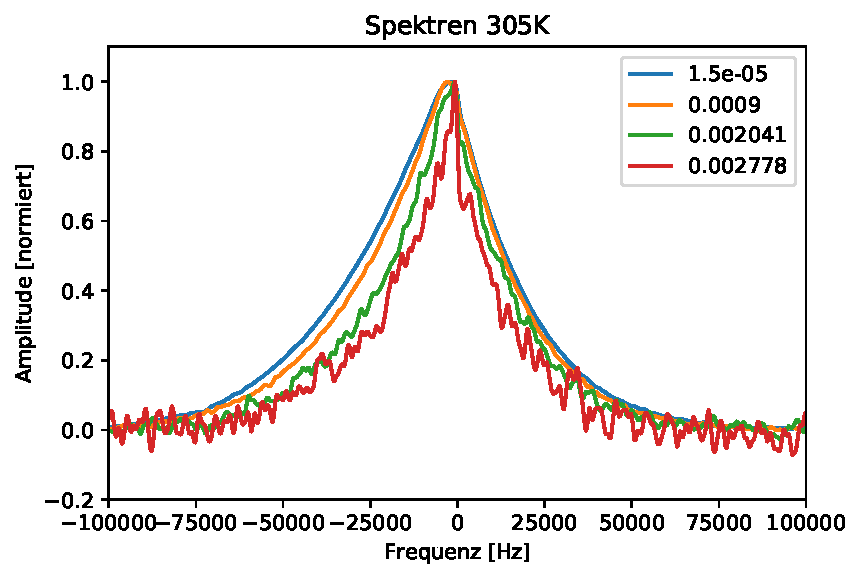
\includegraphics[width=.8\textwidth]{graphics/plots/SPEKDYN/spekdyn_305K.pdf}
	\end{center}
	\caption{Änderung der Linienform der Spektren bei $\SI{305}{\kelvin}$ in Abhängigkeit der Evolutionszeit $t_p$.} \label{fig:res:spekdyn_305K}
\end{figure}
\begin{figure}
	\begin{center}
		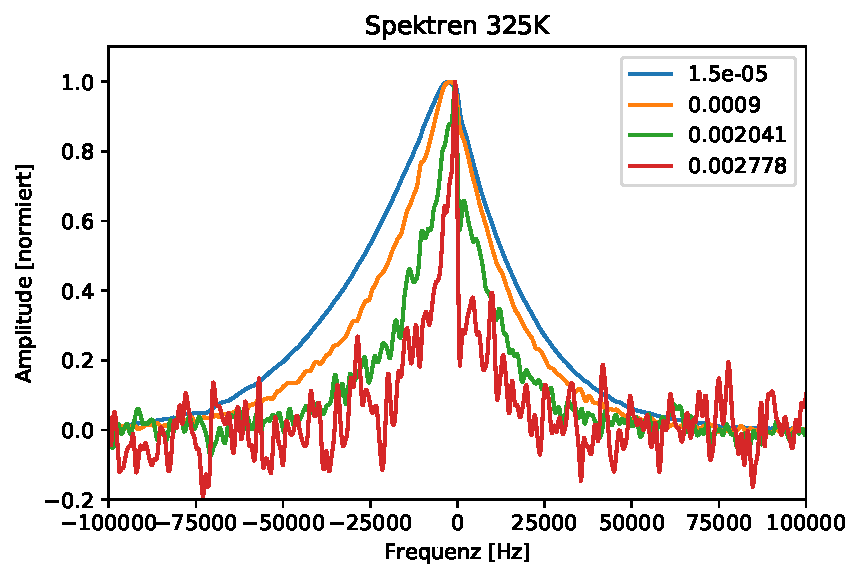
\includegraphics[width=.8\textwidth]{graphics/plots/SPEKDYN/spekdyn_325K.pdf}
	\end{center}
	\caption{Änderung der Linienform der Spektren bei $\SI{325}{\kelvin}$ in Abhängigkeit der Evolutionszeit $t_p$. Im Vergleich zu \ref{fig:res:spekdyn_305K} ist eine deutlich stärkere Verschmälerung zu hohen $t_p$ zu erkennen.} \label{fig:res:spekdyn_325K}
\end{figure}
Alle Spektren wurden mit dem OBI-Spektrometer aufgenommen; dabei wurde ein Hahn-Echo mit variabler Evolutionszeit verwendet und die Spektren mit $\SI{500}{Hz}$ apodisiert.

Zur Untersuchung dieses Phänomens wurde für jede Temperatur die Halbwertsbreite gegen die Evolutionszeit $t_p$ aufgetragen. Da die Spektren bei hohen Pulslängen teils sehr verrauscht sind, wurden die aufgetragengen Evolutionszeiten auf $\SI{2}{\milli s}$ begrenzt. An diese Daten wurden Kohlrausch-Fits angelegt, die als durchgezogene Linien, zusammen mit dem Daten, in Abbildung \ref{fig:res:spekdyn_fits} zu sehen sind.
\begin{figure}
	\begin{center}
		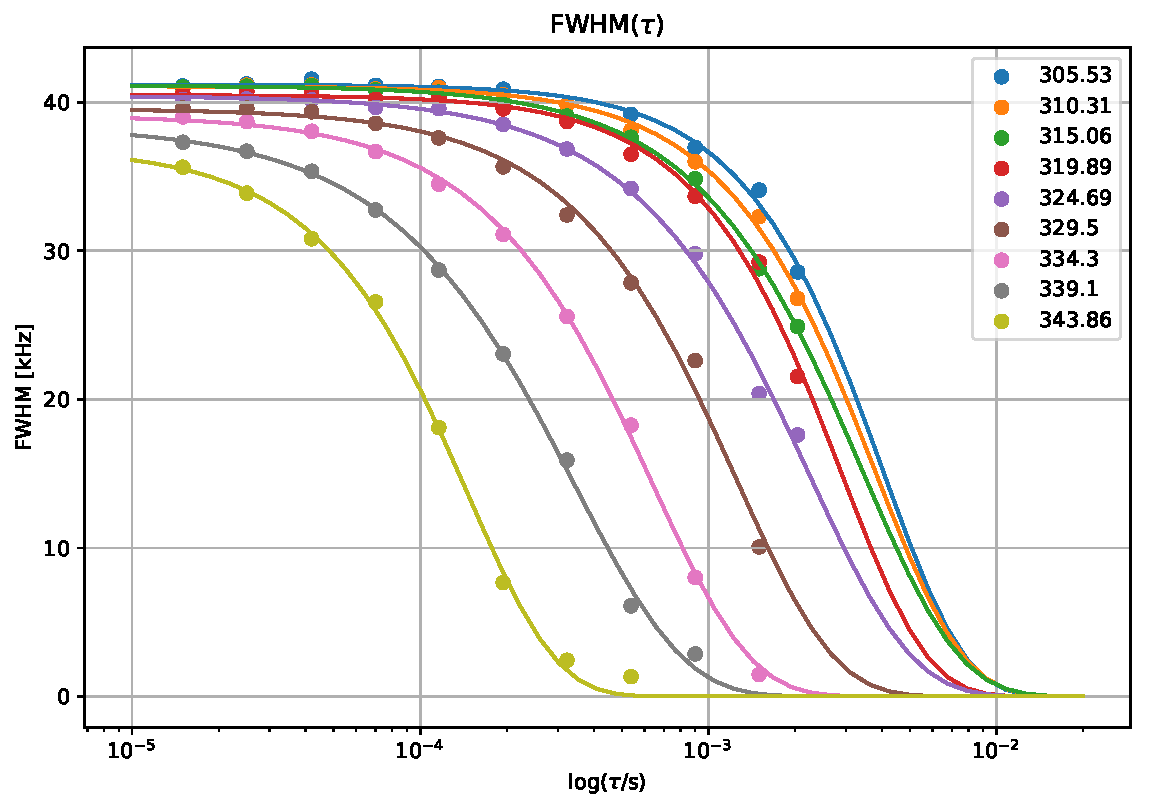
\includegraphics[width=\textwidth]{graphics/plots/SPEKDYN/spekdyn_fits.pdf}
	\end{center}
	\caption{Halbwertsbreiten in Abhängigkeit von $t_p$. An diese Daten wurden Kohlrausch-Fits angelegt, dargestellt als durchgezogene Lininen.} \label{fig:res:spekdyn_fits}
\end{figure}


Es wurde eine weitere, ähnliche Auswertung wurde durchgeführt, wobei anstatt der Halbwertsbreite die Amplitude bei einer bestimmten Frequenz (beispielsweise bei $\SI{-10}{\kilo Hz}$) als Variable genommen wurde. Die Ergebnisse glichen der der Halbwertsbreiten-Betrachtung, waren aber durchgehend mit größeren Unsicherheiten behaftet. Dies lässt sich durch die stark verrauschten Spektren bei hohen Evolutionszeiten erklären, die zu stark schwankenden Amplituden führen, welche wiederum einen guten Fit der Daten schwierig gestalten.

Auswertung ***






\section{Linienform von experimentellen und simulierten CRN-Spektren} \label{section:res:spektren}

Der zweite Abschnitt dieser Arbeit beschäftigt sich mit der Linienform-Untersuchung an CRN-Spektren. Bei der Auswertung von Spektren wurde eine ungewöhnlich erscheinende Verbreiterung der Spektren in einem Temperaturbereich beobachtet, wo, aufgrund von Bewegungsverschmälerung, eher kleinere Halbwertsbreiten zu erwarten wären. Zur Untersuchung der Gegebenheiten wurden, neben einer Vielzahl von experimenteller Spektren, Computer-Simulationen angefertigt, und versucht eine theoretische Erklärung der Daten zu bieten.

\begin{figure}
	\begin{center}
		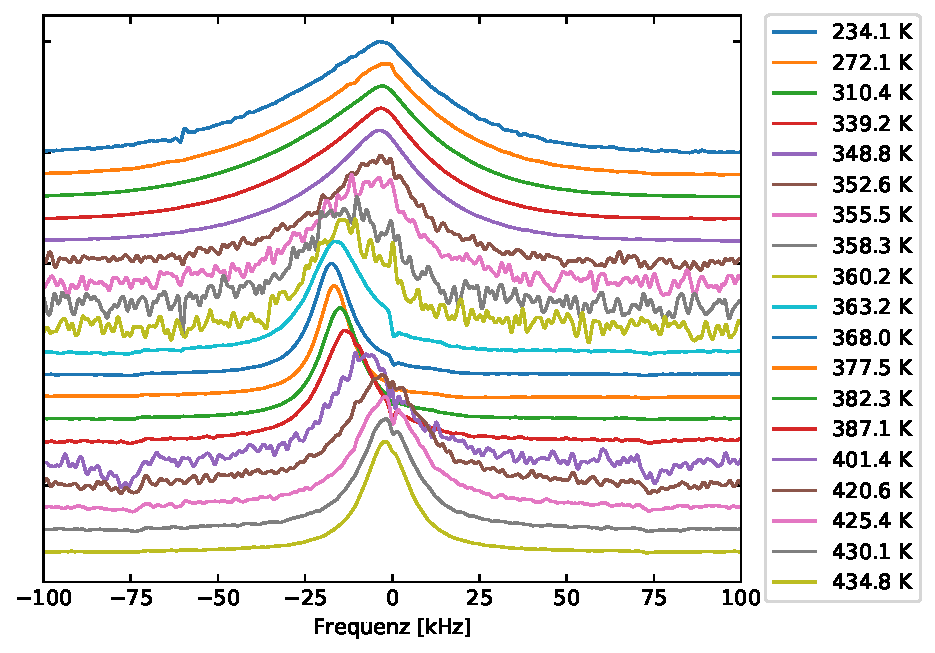
\includegraphics[width=\textwidth]{graphics/plot/spek_lineshape.pdf}
	\end{center}
	\caption{Vergleich der Linienform von am OBI-Spektrometer aufgenommen Spektren.} \label{fig:res:spek_linienform}
\end{figure}
Um eine Übersicht zu schaffen, werden zuerst die Linienformen der Spektren aus den verschiedenen Quellen in Abhängigkeit der Temperatur präsentiert. Abbildung \ref{fig:res:spek_linienform} zeigt die am OBI-Spektrometer aufgenommenen Spektren; die Temperaturen reichen von etwa $\SI{234}{\kelvin}$ bis etwa $\SI{435}{\kelvin}$. Sie wurden mit einem Hahn-Echo mit einer Evolutionszeit von $t_p = \SI{15}{\micro s}$ aufgenommen und mit $\SI{500}{Hz}$ apodisiert. Es wurden je $\SI{8192}{}$ Datenpunkte mit einer Frequenz von $\SI{2}{MHz}$ erstellt. Die Spektren wurden in mehreren Messreihen aufgenommen und stellen eine repräsentative Auswahl dar, die es erlaubt, den Verlauf der Linienform nachzuvollziehen, ohne zu stark an Übersicht zu verlieren.

Bei tiefen Temperaturen ist eine Form zu beobachten, die der des Czjzek-Spektrums aus Kapitel (***) ähnelt. Diese hält sich über weite Temperaturen, von etwa $\SI{235}{\kelvin}$ bis etwa $\SI{350}{\kelvin}$, fast unverändert. Zu höheren Temperaturen ändert sich die Linienform, sie nimmt die einer Lorentz-Funktion an, während die Spektren gleichzeitig schmaler werden und sich der Schwerpunkt zu niedrigeren Frequenzen verschiebt. Diese Bewegung findet ein Ende bei etwa $\SI{367}{\kelvin}$: Zu höheren Temperaturen verbreitern sich die Spektren wieder, ehe sie ab $\SI{410}{\kelvin}$ wieder schmaler werden. Der Schwerpunkt verschiebt sich ab 375K wieder gegen $\SI{0}{Hz}$, wo es ab 400K verweilt. Die Linienform ändert sich nicht mehr.

Es ist auffällig, dass die Qualität der Spektren stark mit der Temperatur schwankt. Zwischen $\SI{235}{\kelvin}$ und $\SI{350}{\kelvin}$, $\SI{363}{\kelvin}$ und $\SI{387}{\kelvin}$, sowie zwischen $\SI{430}{\kelvin}$ und $\SI{435}{\kelvin}$ weisen die Spektren vergleichsweise geringes Rauschen und somit eine glattere Form auf. Das abschnittweise höhere Schwankungen lassen sich durch $T_2$-Minima bei den entsprechenden Temperaturen erklären -- diese sorgen für einen schnellen Abfall des Signals und entsprechend verrauschte Spektren. *** Lorentz

\begin{figure}
	\begin{center}
		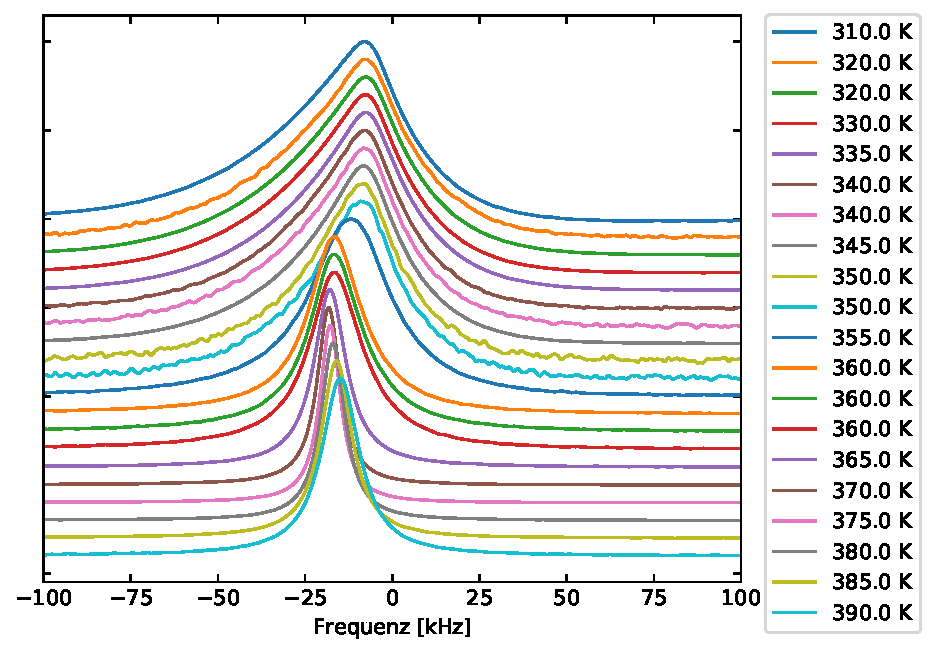
\includegraphics[width=\textwidth]{graphics/plot/bruker_lineshape.pdf}
	\end{center}
	\caption{Vergleich der Linienform von am Bruker-Spektrometer aufgenommen Spektren.} \label{fig:res:bruker_linienform}
\end{figure}
Die am Bruker-Spektrometer aufgenommenen Spektren decken einen Temperaturbereich von $\SI{310}{\kelvin}$ bis $\SI{390}{\kelvin}$ ab, und wurden ebenfalls mit einem Hahn-Echo mit einer Evolutionszeit von $\SI{15}{\micro s}$ erstellt und mit $\SI{500}{Hz}$ apodisiert. Hier wurden je $\SI{4096}{}$ Datenpunkte mit einer Frequenz von $\SI{0.5}{MHz}$ aufgenommen. Da mit diesem Spektrometer weitaus weniger Spektren erstellt wurden als mit dem OBI-Spektrometer können in Abbildung \ref{fig:res:bruker_linienform} alle Spektren präsentiert werden.

Der Verlauf der Linienform gleicht den Beschriebenen in dem entsprechenden Temperaturbereich gut. Es ist das geringe Rauschen der Spektren zu beachten, das, wie auch insbesondere die $T_2$-Daten ein Beleg für hohe Datenqualität des Bruker-Spektrometers in diesem Kontext ist.

Als Ergänzung zu den experimentellen Daten wurden simulierte Spektren angefertigt. Dazu wurde die in Kapitel (***) vorgestellte Simulations-Software verwendet. Es wurden FIDs mit $\SI{4096}{}$ Datenpunkten mit einem Abstand von je $\SI{0.5}{\micro s}$, was einer Frequenz von $\SI{2}{MHz}$ entspricht, aufgenommen. Um einen Mittelwert zu bilden wurden, je nach Spektrum, zwischen $10^{7}$ und $10^{9}$ einzelne Simulationen gemittelt. Als Modell wurde ein isotroper Zufallssprung gewählt, welcher eine Czjzek-Verteilung als Ausgangspunkt hat; dieses war der simulierten Quadrupol-Wechselwirkung zweiter Ordnung ausgesetzt. Zur Bestimmung der Lebensdauer eines bestimmten Zustandes wird eine Exponentialverteilung genutzt, deren Parameter, die Lebenszeit, eine Verknüpfung mit Temperaturen ermöglicht. Es wurde eine Vogel-Fulcher-Funktion für die Lebenszeit mit den Parametern für CRN aus Kapitel (***) verwendet. Zur besseren Vergleichbarkeit werden im Folgenden die Spektren mit den so berechneten Temperaturen anstatt mit den Lebenszeiten referenziert. Die resultierenden Spektren sind in Abbildung \ref{fig:res:sim_linienform} zu sehen.
\begin{figure}
	\begin{center}
		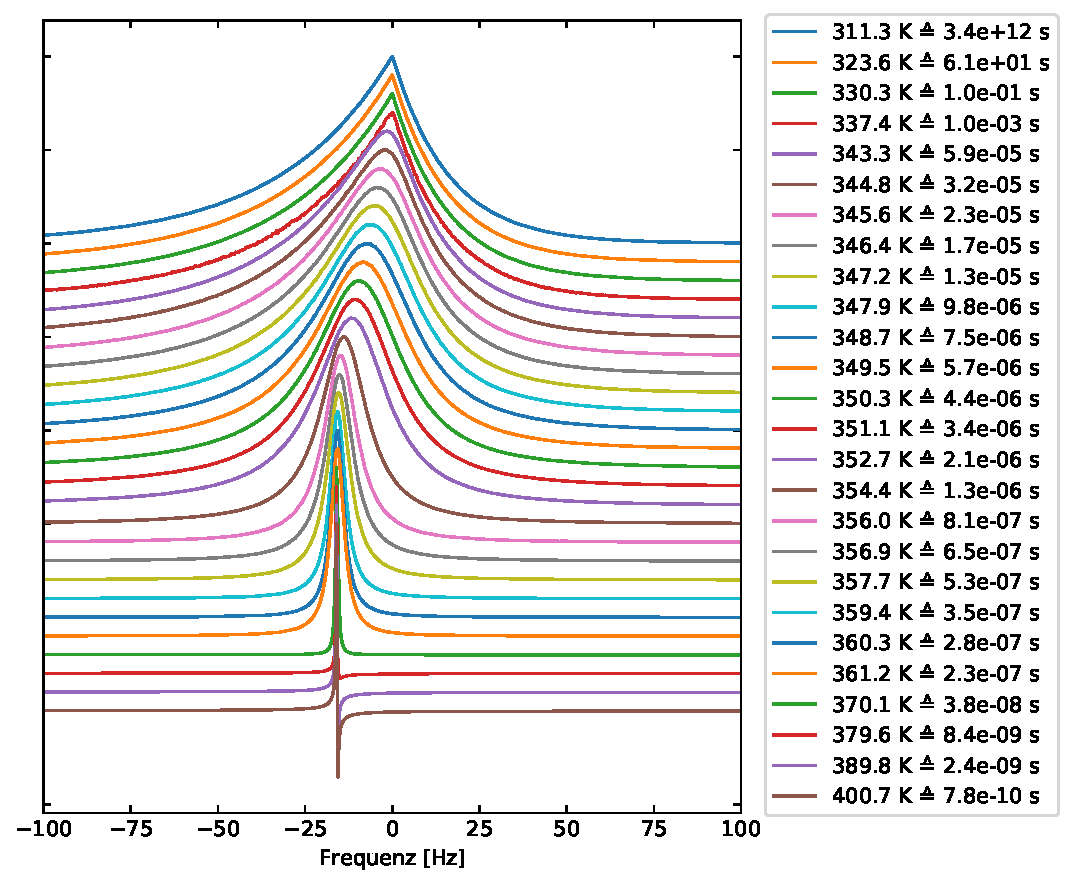
\includegraphics[width=\textwidth]{graphics/plot/sim_lineshape.pdf}
	\end{center}
	\caption{Vergleich der Linienform von mit Simulationen erstellte Spektren. Die angegebenen Temperaturen wurden mithilfe von den in Kapitel \ref{section:res:theorie} beschriebenen $\tau_c$ aus den verwendeten $\tau$ bestimmt.} \label{fig:res:sim_linienform}
\end{figure}

Bei tiefen Temperaturen gleichen die simulierten Spektren den experimentellen. (*** extra Vergleich?) Auch ist der Übergang zur Lorentz-Form, verbunden mit der Verschiebung des Schwerpunkts und Verschmälerung der Spektren bei etwa der gleichen Temperatur von $\SI{350}{\kelvin}$ zu beobachten. Im Gegensatz zu den experimentellen Spektren werden die simulierten Spektren mit steigender Temperatur jedoch immer schmaler und ändern den Schwerpunkt nicht mehr.


Um eine quantitative Behandlung der Spektren zu ermöglichen wurden zwei Messgrößen verwendet: Die Halbwertsbreite (also die Breite auf der Höhe der Hälfte des Maximums) und der Schwerpunkt der Spektren. Um bei den stark verrauschten Spektren des OBI-Spektrometers zwischen $\SI{350}{\kelvin}$ und $\SI{360}{\kelvin}$, und zwischen $\SI{390}{\kelvin}$ und $\SI{430}{\kelvin}$ gut vergleichbare Werte zu erhalten, wurde ein Lorentz-Fit der Form
\begin{align}
	L(f) = \frac{1}{\pi \gamma} \cdot \frac{\gamma^2}{\gamma^2 + (f - f_0)^2} \label{eqn:res:lorentz}
\end{align}
mit einer least-squares-Methode an die Spektren angelegt. So entspricht $2 \gamma$ der Halbwertsbreite und das Maximum $f_0$, aufgrund der Symmetrie der Funktion, dem Schwerpunkt. Die so gewonnenen Halbwertsbreiten sind in Abbildung \ref{fig:res:spek_fwhm} zu sehen.
\begin{figure}
	\begin{center}
		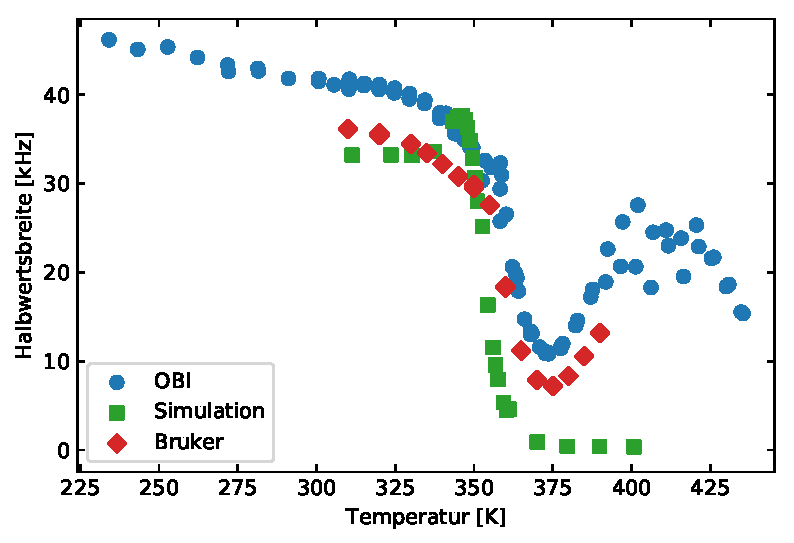
\includegraphics[width=.9\textwidth]{graphics/plot/fwhm.pdf}
	\end{center}
	\caption{Die Halbwertsbreite der Spektren. Blaue und rote Symbole kennzeichnen am OBI- bzw. Bruker-Spektrometer aufgenommene Spektren, grüne Symbole stammen von simulierten Spektren. Der auffälligste Unterschied zwischen experimentellen und simulierten Spektren ist das zusätzliche Maximum bei hohen Temperaturen bzw. das Fehlen dessen.} \label{fig:res:spek_fwhm}
\end{figure}

Es ist zu erkennen, dass die Werte der Halbwertsbreite etwa dem entsprechen, was nach einer Betrachtung der Spektren zu erwarten wäre: Von einem breiteren Spektrum bei niedrigen Temperaturen gehen die Breiten zu einem Minimum bei etwa $\SI{375}{\kelvin}$ über, um nach einem Maximum bei etwa $\SI{400}{\kelvin}$ erneut abzufallen.

Dieser Verlauf der am OBI-Spektrometer aufgenommenen Spektren folgen auch die Halbwertsbreiten der am Bruker-Spektrometer produzierten Daten. Letztere liegen allerdings konstant bei niedrigeren Werten. Das Verhältnis entspricht aber auch nicht durchgehend dem Verhältnis $4:3$, was die unterschiedlichen Larmorfrequenzen suggestieren würden; es liegt bei tiefen Temperaturen etwas niedriger und bei höheren Temperaturen etwas höher. So ist im Bereich zwischen $\SI{310}{\kelvin}$ und $\SI{350}{\kelvin}$ ein Verhältnis von etwa $\SI{1.15}{}:1$ zu finden, zwischen $\SI{360}{\kelvin}$ und $\SI{390}{\kelvin}$ ein Verhältnis von $\SI{1.45}{}:1$ bis $\SI{1.55}{}:1$.

Der Verlauf der Halbwertsbreiten der simulierten Spektren unterscheidet sich deutlich von dem der experimentellen Spektren. Während der grobe Verlauf übereinstimmt -- von breiten Spektren bei tiefen Temperaturen zu schmalen Spektren bei höheren Temperaturen -- sind starke Abweichungen zu sehen. Die simulierten Spektren werden zu höheren Temperaturen zunehmend schmaler, während die experimentellen Spektren ein weiteres Maximum aufweisen. Zudem ist ein Maximum der Halbwertsbreite der simulierten Spektren bei etwa $\SI{345}{\kelvin}$ beobachten, während die Halbwertsbreite der experimentellen Spektren einen fließenden Übergang der Breite von hohen zu tiefen Temperaturen zeigen.

Es sollte darauf aufmerksam gemacht werden, dass die Halbwertsbreite stark von der Form der Spitze beeinflusst wird, welche das Maximum und damit die Hälfte des Maximums bestimmt. Sind, wie bei den simulierten Spektren, extrem gut definierte Maxima zu sehen, drückt dies den Wert der Halbwertsbreiten im Vergleich zu den experimentellen Halbwertsbreiten nach unten. Dies erklärt den Abfall der Halbwertsbreiten der simulierten Spektren zu tieferen Temperaturen: Hier sind die scharfe Spitzen der Czjzek-Spektren gut ausgeprägt, sodass die Halbwertsbreite der Spektren beim Übergang zur abgerundeten Lorentz-Form ein Maximum durchläuft. Die experimentellen Spektren hingegen zeigen aufgrund von experimentellen Beschränkungen wie der Auflösung -- und möglicherweise durch weitere Effekte -- bei niedrigeren Temperaturen keine perfekte Spitze und daher auch keinen Peak in der Halbwertsbreite beim Übergang zur Lorentz-Form.


Messungen an einem $\SI{600}{MHz}$-Spektrometer wären hilfreich um Aussagen über die chemische Verschiebung machen zu können. *** 



In Abbildung \ref{fig:res:spek_mean} sind die Schwerpunkte der Spektren aufgetragen. Diese wurden mit Hilfe von numerischer Integration nach der Simpsonregel bestimmt. Bei stark verrauschten Spektren, wo dieses Vorgehen wenig Erfolg verspricht -- es wird eher der Schwerpunkt der Schwankungen bestimmt als des Signals --, wurden wieder Lorentz-Fits ausgenutzt, deren Parameter $f_0$ der Schwerpunkt ist.
\begin{figure}
	\begin{center}
		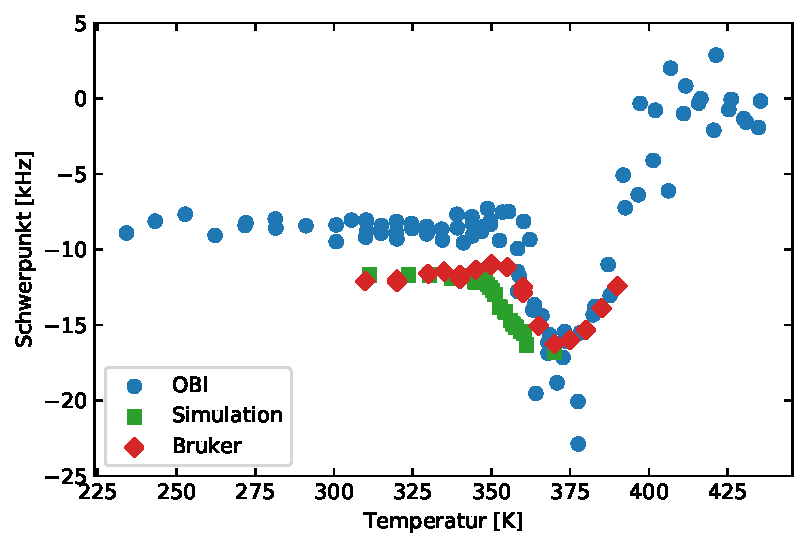
\includegraphics[width=.9\textwidth]{graphics/plot/mean.pdf} 
	\end{center}
	\caption{Die Halbwertsbreite der Spektren. Blaue und rote Symbole kennzeichnen am OBI- bzw. Bruker-Spektrometer aufgenommene Spektren, grüne Symbole stammen von simulierten Spektren. Während der Schwerpunkt der experimentellen Spektren zu hohen Temperaturen gegen $\SI{0}{\kilo Hz}$ geht, verbleibt der Schwerpunkt der simulierten Spektren bei etwa $\SI{-16}{\kilo Hz}$.} \label{fig:res:spek_mean}
\end{figure}

Allen drei Kurvenverläufe ist gleich, dass sie bei tieferen Temperaturen bis etwa $\SI{360}{\kelvin}$ einen konstanten Wert zeigen, ehe sich der Schwerpunkt zu niedrigeren Frequenzen von etwa $\SI{-16}{\kilo Hz}$ verschiebt, was mit dem Übergang von der Czjzek-Form des Spektrums zur Lorentz-Form einhergeht. Die spezifischen konstanten Werte der tieferen Temperaturen unterscheiden sich jedoch zwischen den Daten des OBI-Spektrometers mit einem Schwerpunkt von etwa $\SI{-8}{\kilo Hz}$, und den Daten des Bruker-Spektrometers und der Simulation mit einem Schwerpunkt von etwa $\SI{-12}{\kilo Hz}$. Ab etwa $\SI{375}{\kelvin}$ ist eine Bewegung des Schwerpunkts der experimentellen Spektren zum Nullpunkt zu erkennen, die die Spektren des OBI-Spektrometers aufgrund des größeren abgedeckten Temperaturbereichs auch erreichen. Die simulierten Spektren verbleiben jedoch bei dem Wert von $\SI{-16}{\kilo Hz}$, der bei $\SI{370}{\kelvin}$ erreicht wird.


Auch hier ist einschränkend zu sagen, dass die Werte der Schwerpunkte aufgrund von externen Faktoren instabil sind, mehr noch als die Halbwertsbreiten. Wie in Kapitel \ref{section:exp:weiterverarbeitung} erwähnt, wird eine Phasenanpassung des Real- und Imaginärteils durchgeführt, um ein maximales Signal zu garantieren und mögliche Schwankungen der Phase durch experimentelle Einflüsse auszugleichen. Allerding kann eine Abweichung von $\pm \SI{1}{\degree}$ vom Optimalwert unter den schlechtesten Umständen eine Verschiebung des Schwerpunkts um $\SI{1}{\kilo Hz}$ bewirken. Diese Empfindlichkeit gegenüber kleinen Änderungen bedeutet, dass Schwankungen der dargestellten Werte nicht auszuschließen ist; die groben Merkmale der Kurvenverläufe können aber leicht durch eine Betrachtung der Spektren bestätigt werden.




\section{Vergleich von CRN-Spektren mit theoretischen Überlegungen} \label{section:res:theorie}

Die experimentellen Ergebnisse sollen mit den theoretischen Überlegungen vergleichen werden. Dazu wurden die in Kapitel \ref{section:theo:eckert} beschriebenen Funktionen für $T_1$, Halbwertsbreite und Schwerpunkt verwendet. Um eine Übereinstimmung zur Theorie feststellen zu können, müssen sich alle Datensätze mit dem gleichen Satz geteilter Parameter beschreiben lassen. Im Falle der Spektraldichte $J(\omega)$ ist dies $C_Q$; für $J_\text{CC}$ und $J_\text{CD}$ sind $\alpha$ bzw. $\gamma$ zusätzliche Parameter.

Für den Parameter $\eta$ der Spektraldichten wurde $\eta^2 = 42 - 24 \sqrt{3} \approx \SI{0.43}{}$ \cite{caer} verwendet. Nach \cite{PIMENOV199793} wird für CRN für die Korrelationszeit $\tau_c$ ein Vogel-Fulcher-Gesetz
\begin{align}
	\tau_c = \tau_{co} \exp \left( \frac{D T_\text{VF}}{T-T_\text{VF}} \right)
\end{align}
mit dem strength index $D = \SI{3.5}{}$, der Vogel-Fulcher-Temperatur $T_\text{VF} = \SI{294}{K}$ und dem Frequenzfaktor $\tau_{co} = \SI{5.1e-14}{s}$ angenommen. Diese Werte wurden durch *** bestimmt.

Das $T_1$-Minimum kann in den Daten bei etwa $T_\text{min} = \SI{390}{K}$ gefunden werden; die Larmorfrequenz liegt bei $\omega_L = 2\pi \cdot \SI{97.1722}{MHz}$, was bedeutet, dass bei $T_\text{min}$ gilt $\tau_c \approx \frac{\SI{0.61}{}}{\omega_L} \approx \SI{1.0}{\nano s}$. Vergleicht man das Vogel-Fulcher-Gesetz mit diesem Punkt, lässt sich erkennen, dass eine gute Übereinstimmung vorliegt.
\begin{wrapfigure}{r}{0.5\textwidth}
	\vspace{-20pt}
	\begin{center}
		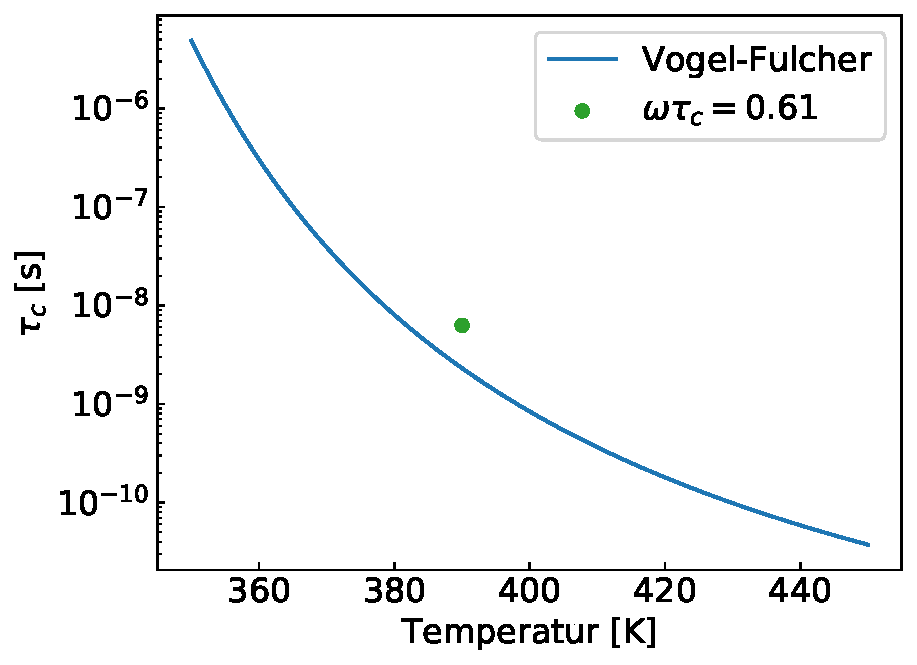
\includegraphics[width=0.49\textwidth]{graphics/zwischenbericht/tau_c_arrhenius_vogel_fulcher.pdf}
	\end{center}
	\vspace{-20pt}
	\caption{Vergleich von Zeitkonstante aus $T_1$-Minimum mit Vogel-Fulcher-Gesetz \label{fig:korrelationszeiten} ***}
\end{wrapfigure}

Ein Vergleich mit den Parametern $D = \SI{4.72}{}$, $T_\text{VF} = \SI{285}{K}$ und $\tau_{co} = \SI{1.15e-14}{s}$ nach \cite{crn_augsburg} ist in Abbildung \ref{fig:res:theorie_j} zu sehen. Während leichte Unterschiede zu erkennen sind, ändert sich das Gesamtbild wenig, weswegen sich diese Ausführungen auf den ersten Parametersatz beschränken.




Führt man zunächst einen Vergleich der Halbwertsbreiten mit der Theorie durch, lässt sich leicht feststellen, dass signifikante Unterschiede zu beobachten sind: Die gemessenen Halbwertsbreiten sind ab $\SI{360}{\kelvin}$ aufwärts deutlich größer als vorhergesagt. Dies liegt am Einfluss des kurzen $T_1$ von etwa $\SI{50}{\micro s}$, welches mit der zusätzlich Relaxation zur Verbreiterung des Spektrums beiträgt.

Um einen Vergleich mit der Theorie dennoch durchführen zu können, wurde versucht den Einfluss von $T_1$ rechnerisch zu eliminieren. Im Bereich des Einflusses lassen sich die Spektren gut mit einem Lorentz-Fit (vgl. Gleichung \eqref{eqn:res:lorentz}) näheren. Die Fouriertransformierte hiervon ist eine gedämpfte Schwingung mit der Halbwertsbreite $2 \gamma = a/\pi$:
\begin{align}
	h(t) & = \exp{(-a |t|)} \cos{(2 \pi f_0 t)}                              \\
	H(t) & = \int_{-\infty}^{\infty} h(t) \text{d} t                         \\
	H(f) & = \frac{2}{a} \cdot \frac{(a/2\pi)^2}{((a/2\pi)^2) + (f - f_0)^2}
\end{align}

Diese gedämpfte Schwingung soll durch eine normierte Kohlrausch-Funktion, welche für Fits an $T_1$ verwendet werden kann, geteilt werden.
\begin{align}
	f(t) = \exp{\left( {\left(\frac{-t}{T_1} \right)}^\beta \right) }
\end{align}
Für eine vereinfachte Rechnung wird hier wird $\beta = 1$ angenommen, was in der Regel eine annehmbare Näherung darstellt. Wird der Quotient der Funktionen zurück in den Frequenzraum transformiert, ergibt sich die modifizierte Halbwertsbreite $2\gamma = 2(\gamma_0 - \frac{1}{\pi T_1})$.

Dies bedeutet, dass für die Korrektur lediglich die schon vorliegenden Halbwertsbreiten mit $T_1$-Werten der passenden Temperaturen modifiziert werden müssen. Diese wurden aus den durchgeführten $T_1$-Messungen gewonnen. Die Ergebnisse sind in Abbildung \ref{fig:res:spek_fwhm_t1} zu sehen.
\begin{figure}
	\begin{center}
		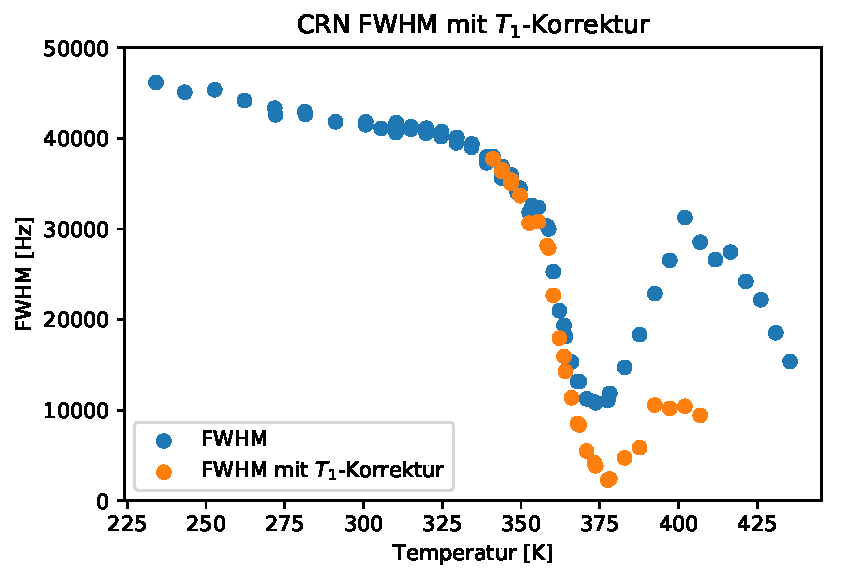
\includegraphics[width=\textwidth]{graphics/plots/SPEK/spek_t1korr.pdf}
	\end{center}
	\caption{Halbwertsbreite der OBI-Spektren in blau, mit der beschriebenen $T_1$-Korrektur in orange.} \label{fig:res:spek_fwhm_t1}
\end{figure}

Es ist zu erkennen, dass $T_1$ einen großen Einfluss auf die Halbwertsbreite hat und die entsprechend angepassten Halbwertsbreiten deutlich geringere Werte aufweisen. Bei Temperaturen über $\SI{410}{\kelvin}$ konnte keine Korrektur vorgenommen werden, weil die $T_1$-Werte in diesem Temperaturbereich zu stark streuen um aussagekräfige Daten zu produzieren.




Es wurden die am OBI- und am Bruker-Spektrometer aufgenommenen Daten getrennt untersucht, da durch die unterschiedlichen Larmorfrequenzen abweichende Ergebnisse der theoretischen Kurven zu erwarten sind. Bei den Halbwertsbreiten wurde der $T_1$-Einfluss nach der beschriebenen Methode berücksichtigt.



Die aufgenommenen Spektren unterstützen eine biexponentielle Interpretation wie in \eqref{eqn:trans_relax} nur schwerlich, daher wurde lediglich der deutlich zu beobachtende Anteil des Zentralübergangs, $\Delta_c$ und $\omega_c^{(2)}$, für die entsprechenden FWHM- bzw. Schwerpunkts-Daten betrachtet. Für die $T_1$-Daten wird Formel \eqref{eqn:bpp} verwendet. Alle Fits wurden manuell erstellt.



Zunächst sollen die Daten des OBI-Spektrometers vergleichen werden. Bei den $T_1$ Werten soll erwähnt werden, dass die Werte bei hohen Temperaturen mit starken Unsicherheiten belegt sind (vlg. Abbildung \ref{fig:res:T_1}) -- entsprechende Indikatoren wurden hier für eine bessere Übersicht ausgelassen.

Für die Spektraldichte $J_\text{BPP}$ kann bei höheren Temperaturen, wie in Abbildung \ref{fig:res:theorie_j} zu sehen, mit dem Parameter $C_Q = \SI{3.6}{MHz}$ eine vergleichsweise gute Übereinstimmung für die Halbwertsbreiten und die Schwerpunkte erreicht werden. Zu tieferen Temperaturen gibt es jedoch gravierende Abweichungen. Für die stark ansteigenden Werte der Halbwertsbreite können anisotrope Effekte vermutet werden, deren Einfluss durch diese isotrope Theorie nicht abgedeckt wird. Gründe für die Abweichungen der Schwerpunkte sind noch offen -- diese Effekt wird jedoch gleichermaßen in experimentellen als auch simulierten Spektren beobachtet, was bedeutet, dass der Effekt vermutlich auf die von der Simulation berücksichtigten Wechselwirkungen eingeschränkt werden kann.
\begin{figure}
	\begin{center}
		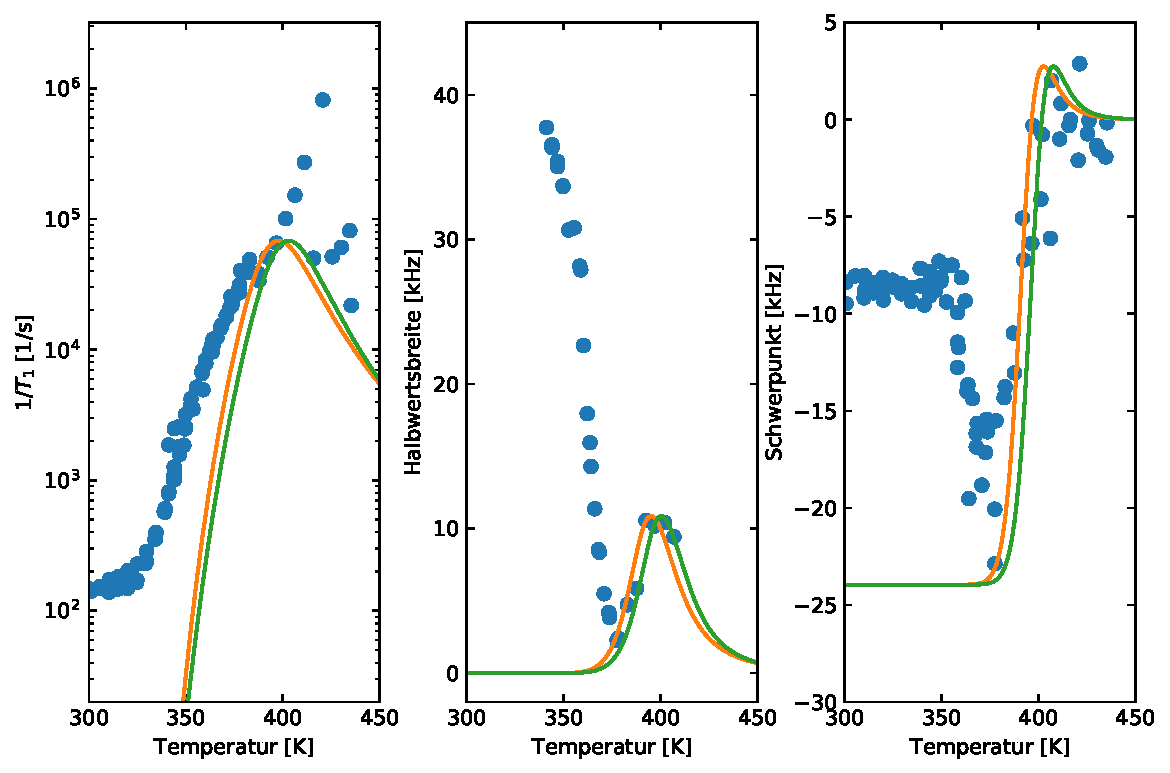
\includegraphics[width=\textwidth]{graphics/plot/OBI_J_02.pdf}
	\end{center}
	\caption{Vergleich von $T_1$, Halbwertsbreite und Schwerpunkt der OBI-Daten in blau. In orange die Theorie-Kurve mit Spektraldichte $J_\text{BPP}$ mit Parametern nach \cite{PIMENOV199793}, in grün mit Parametern nach \cite{crn_augsburg}.} \label{fig:res:theorie_j}
\end{figure}

Es kann eine grobe Vereinbarkeit der Theorie mit $T_1$-Werten im Maximum der Kurve erreicht werden, die Flanken unterscheiden sich jedoch deutlich. Da die Form der Theoriekurve mit der Spektraldichte $J_\text{BPP}$ unveränderlich ist, ist es schwerlich möglich, eine zufriedenstellende Übereinstimmung zu erreichen. Abhilfe schaffen könnten andere Spektraldichten -- dies soll im Folgenden untersucht werden.

Für die Spektraldichten $J_\text{CC}$ (Abbildung \ref{fig:res:theorie_j_cc} und $J_\text{CD}$ (Abbildung \ref{fig:res:theorie_j_dc}) lagen die für die theoretische Berechnung der Schwerpunkte benötigten Imaginärteile $Q_\text{CC}$ und $Q_\text{CD}$, weswegen für diese auf die Spektraldichte $J_\text{BPP}$ zurückgegriffen wurde. Für die Schwerpunkte kann der Vergleich daher nur als grobe Idee verstanden werden.
\begin{figure}
	\begin{center}
		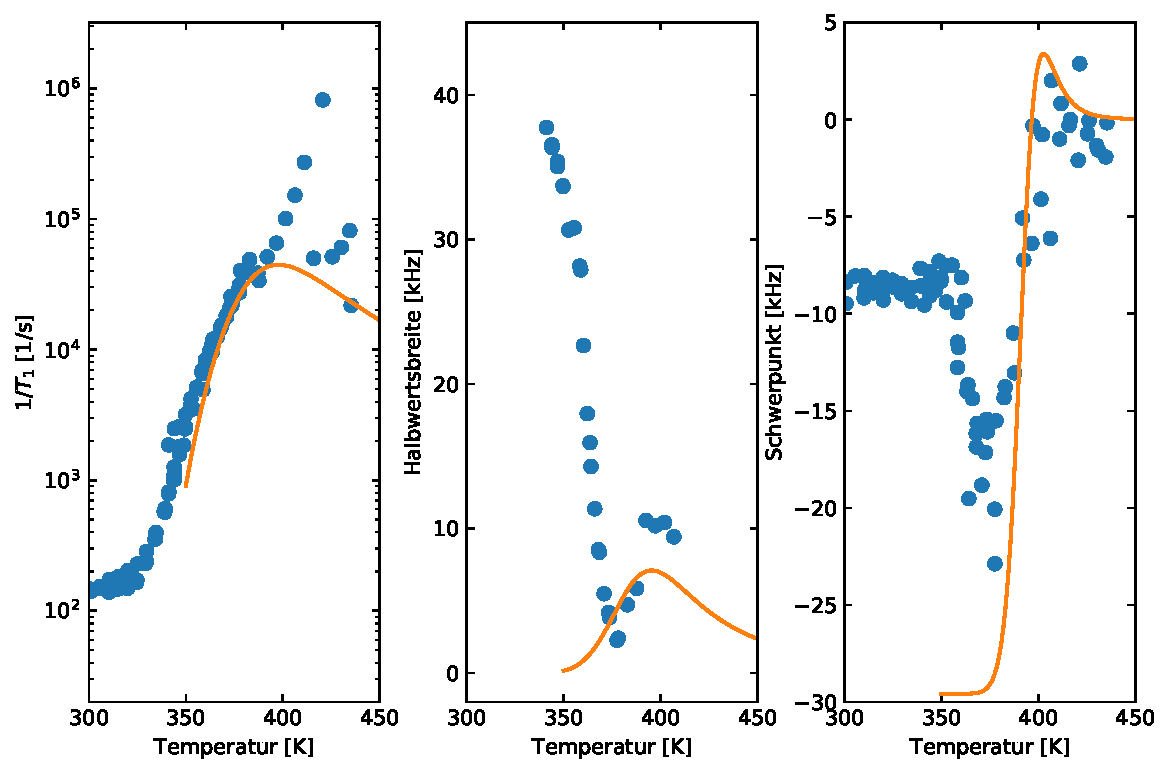
\includegraphics[width=\textwidth]{graphics/plot/OBI_J_cc_01.pdf}
	\end{center}
	\caption{Vergleich von $T_1$, Halbwertsbreite und Schwerpunkt der OBI-Daten in blau. In orange die Theorie-Kurve mit Spektraldichte $J_\text{CC}$ mit Parametern nach \cite{PIMENOV199793}.} \label{fig:res:theorie_j_cc}
\end{figure}
\begin{figure}
	\begin{center}
		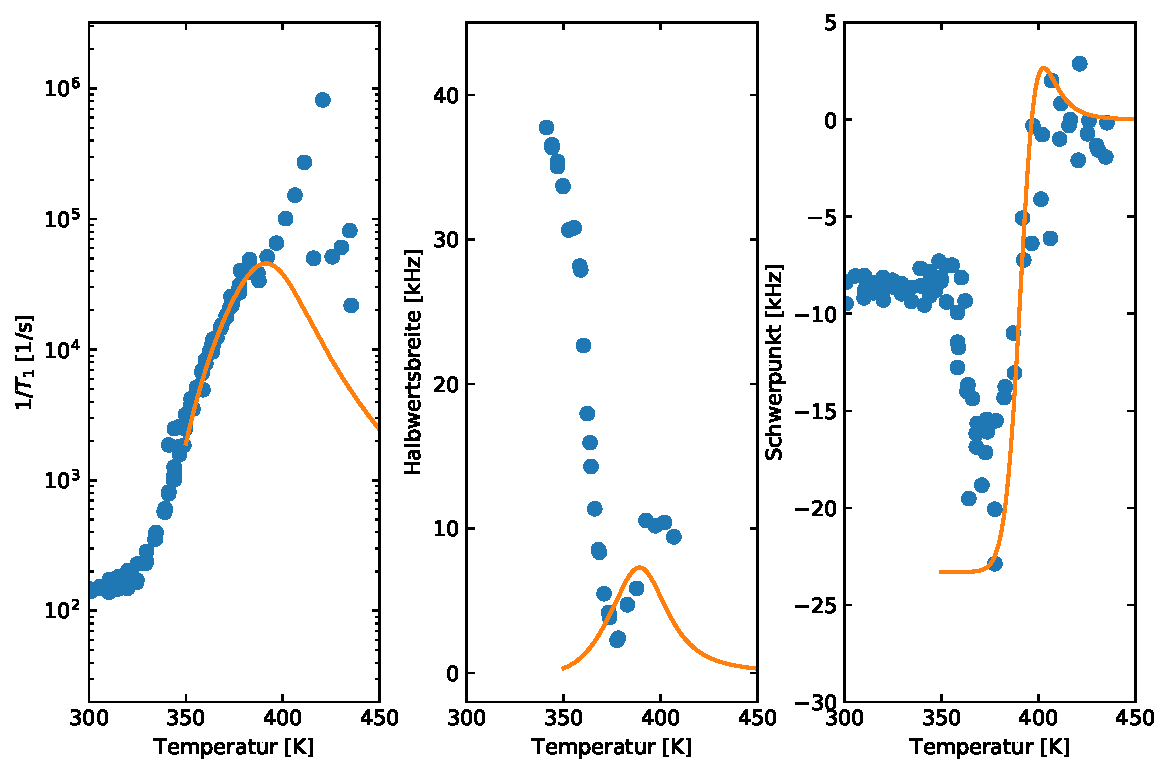
\includegraphics[width=\textwidth]{graphics/plot/OBI_J_dc_01.pdf}
	\end{center}
	\caption{Vergleich von $T_1$, Halbwertsbreite und Schwerpunkt der OBI-Daten in blau. In orange die Theorie-Kurve mit Spektraldichte $J_\text{CD}$ mit Parametern nach \cite{PIMENOV199793}.} \label{fig:res:theorie_j_dc}
\end{figure}

Für $J_\text{CC}$ und $J_\text{CD}$ können mit den Parametern $C_Q = \SI{4.0}{MHz}$ und $\alpha = \SI{0.6}{}$ bzw. $C_Q = \SI{3.6}{MHz}$ und $\gamma = \SI{0.46}{}$ gute Übereinstimmungen für $T_1$ beobachtet werden -- zumindest bis zu einer Temperatur von etwa $\SI{350}{\kelvin}$. Für $J_\text{CD}$ scheint es zudem für Temperaturen über $\SI{400}{K}$ Abweichungen zu geben. Bessere Vereinbarkeit mit $T_1$-Werten kommt in beiden Fällen auf Kosten der vergleichsweise guten Übereinstimmung für Halbwertsbreite und Schwerpunkt, die mit $J_\text{BPP}$ erreicht werden konnten: Während für $J_\text{CC}$ die Schwerpunkte stark abweichen, ist dies bei $J_\text{CD}$ für die Halbwertsbreiten der Fall. Es bleibt festzuhalten, dass insgesamt eine gute Übereinstimmung mit der Theorie gezeigt werden konnte; es kann jedoch keine Spektraldichte besonders vorteilhaft hervorgehoben werden.

Für den Vergleich der Daten des Bruker-Spektrometers ist Ähnliches zu beobachten. Dabei fällt es hier aber schwerer, definitive Aussagen zu treffen, da der eingeschränkte Temperaturbereich nur einen bedingten Vergleich zulässt. Abbildung *** zeigt die Daten zusammen mit Theoriekurven basierend auf der Spektraldichte $J_\text{BPP}$ mit dem Parameter $C_Q = \SI{3.45}{MHz}$. Dabei ist zu sehen, dass die Daten im gleichen Maße Übereinstimmung und Unterschiede aufzeigen.
\begin{figure}
	\begin{center}
		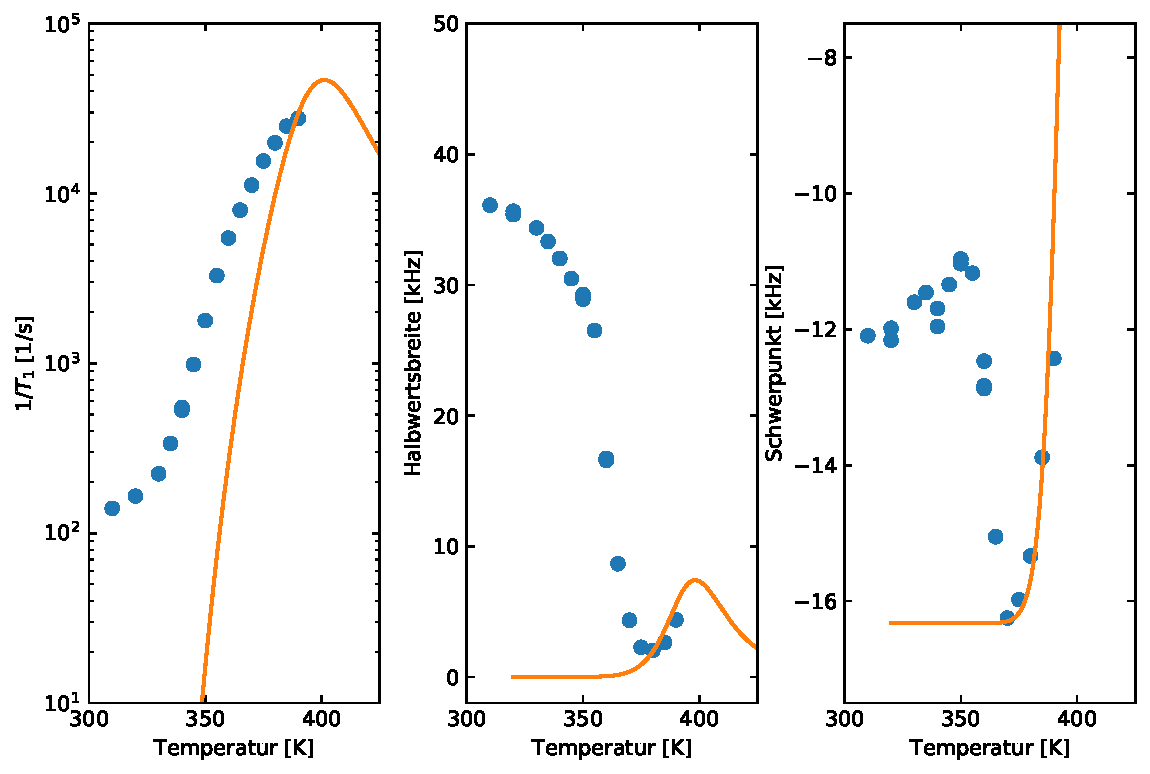
\includegraphics[width=\textwidth]{graphics/plot/Bruker_J_01.pdf}
	\end{center}
	\caption{Vergleich von $T_1$, Halbwertsbreite und Schwerpunkt der Bruker-Daten in blau. In orange die Theorie-Kurve mit Spektraldichte $J_\text{BPP}$ mit Parametern nach \cite{PIMENOV199793}.} \label{fig:res:theorie_bruker}
\end{figure}





***


Werden die resultierenden Zeitkonstanten zusammen mit $T_2$ aufgetragen, zeigt sich eine hohe Ähnlichkeit, was vermuten lässt, dass mit der Methode $T_2$ gemessen wurde.
\begin{figure}
	\begin{center}
		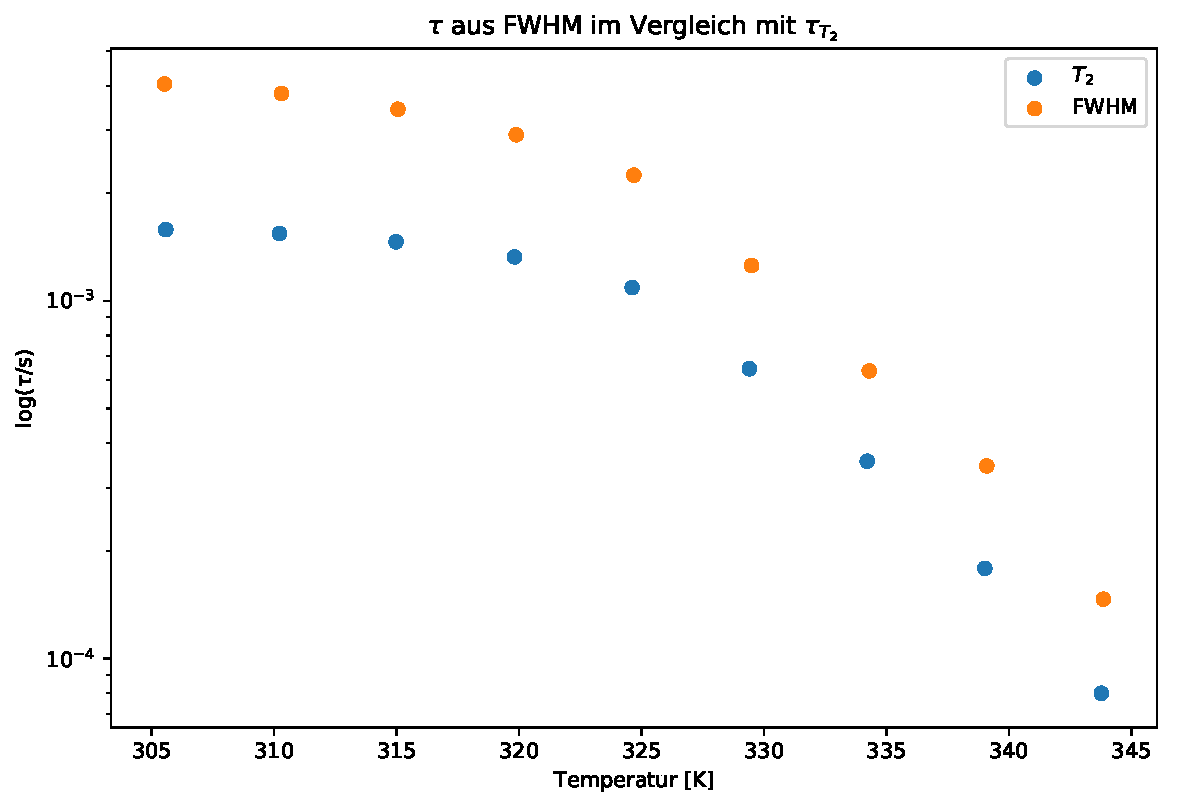
\includegraphics[width=\textwidth]{graphics/plots/SPEKDYN/spekdyn_t2.pdf}
	\end{center}
	\caption{$\tau$ aus FWHM im Vergleich mit $T_2$} \label{fig:res:spekdyn_t2}
\end{figure}
